\chapter{Results and Discussions}
\label{chap:results}

In the following, the results obtained from the finite element simulation using different setups are discussed and compared to the outer pressure field measurement.

\section{Comparison of simulation and measurement results}



\begin{figure}%[H] do not start with figure after a section heading!
	% Einheiten: "quantity" in "unit", nicht [unit] !
	\centering
	\begin{subfigure}[b]{0.49\textwidth}
		\centering
		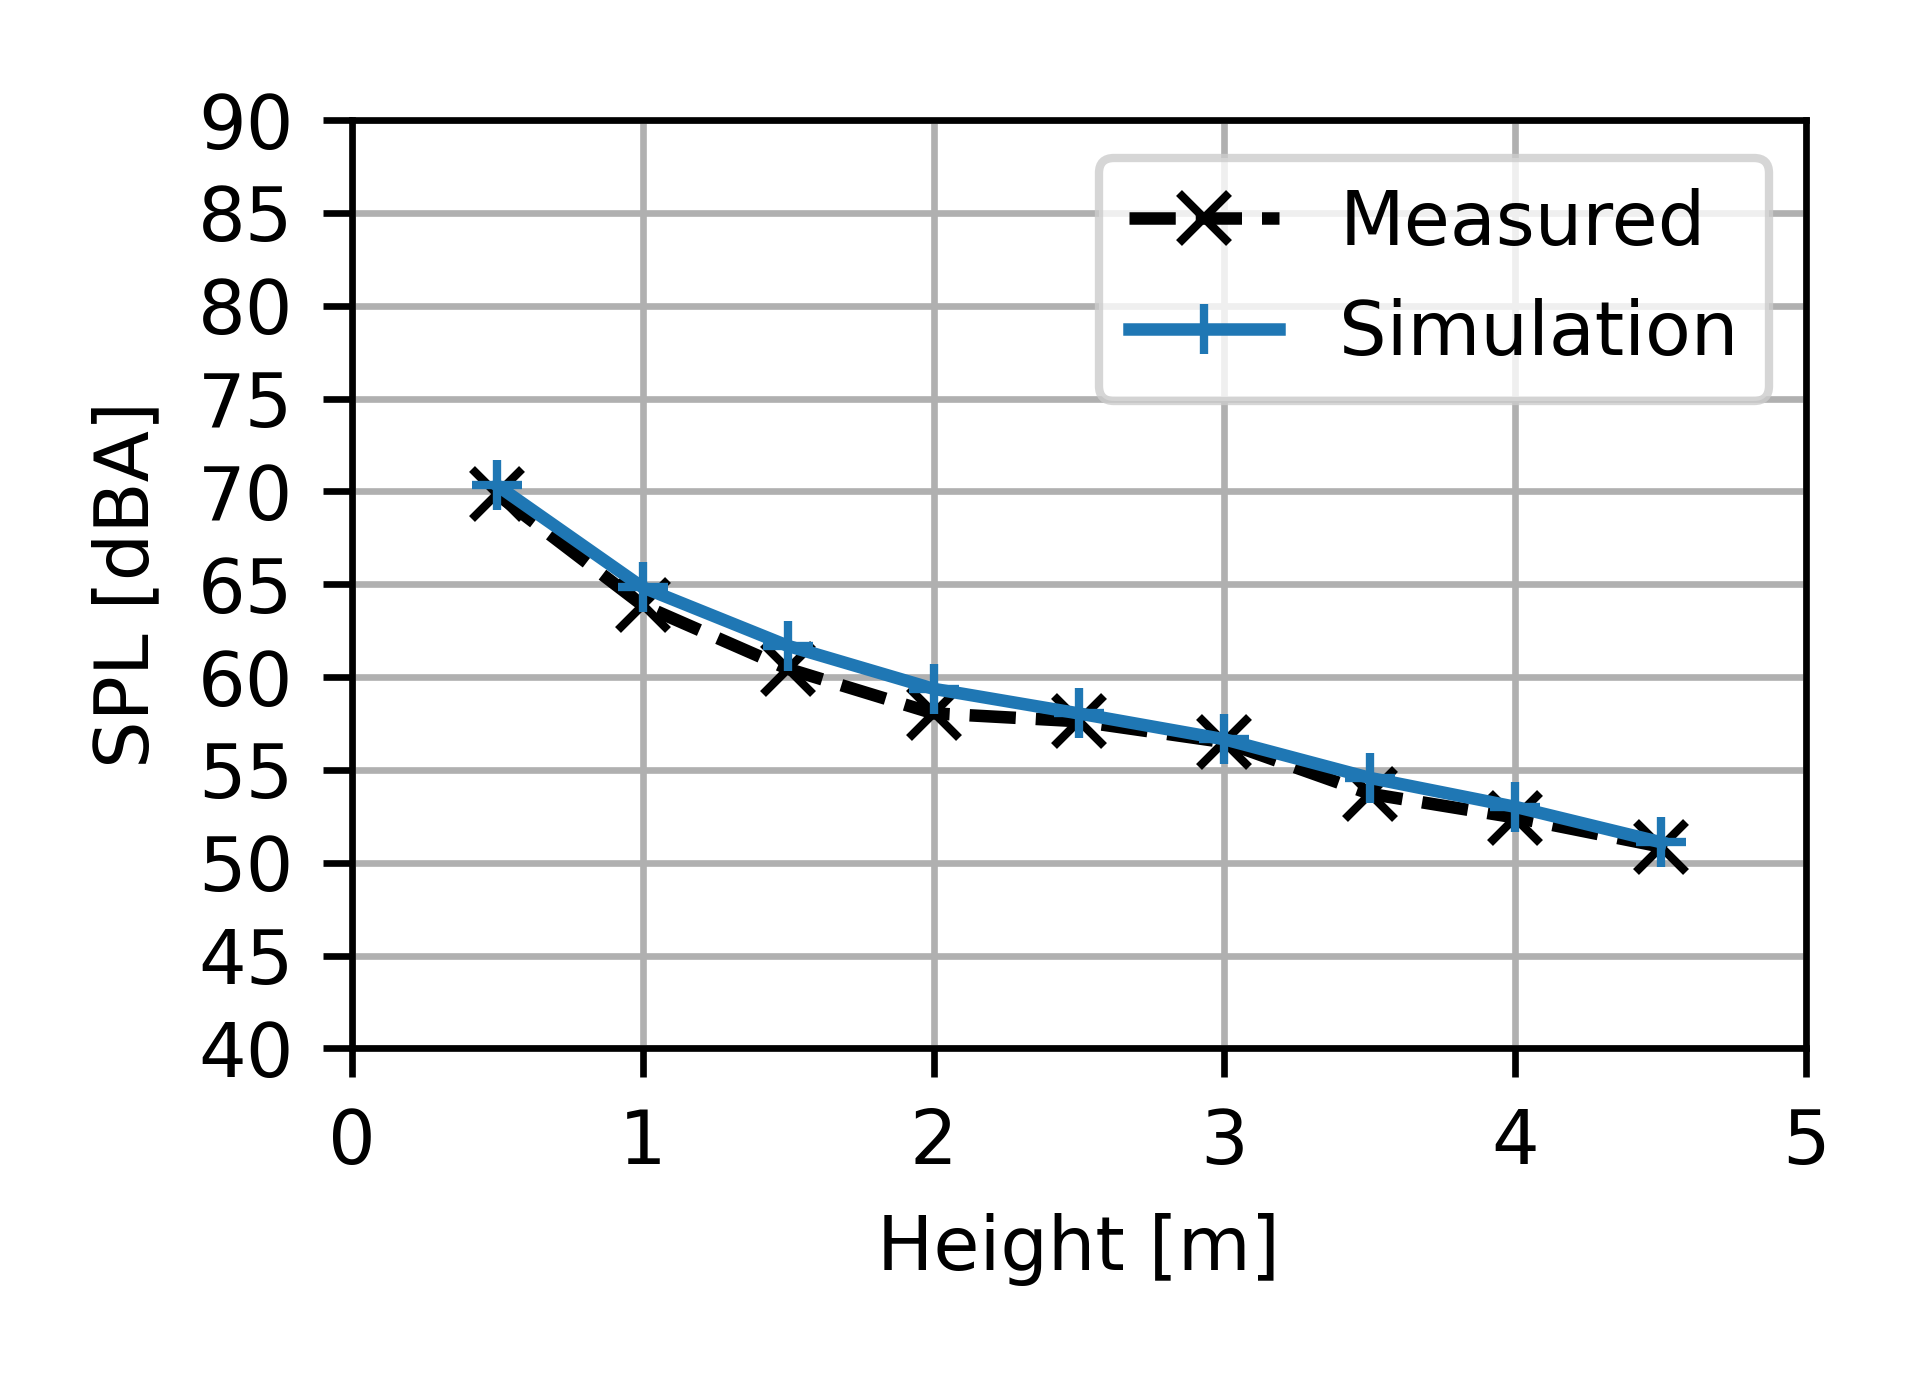
\includegraphics{fig/chap5/initial_model/third_octave_over_height/125_Hz.png}
		\caption{\SI{125}{\hertz}}
	\end{subfigure}
	\hfill
	\begin{subfigure}[b]{0.49\textwidth}
		\centering
		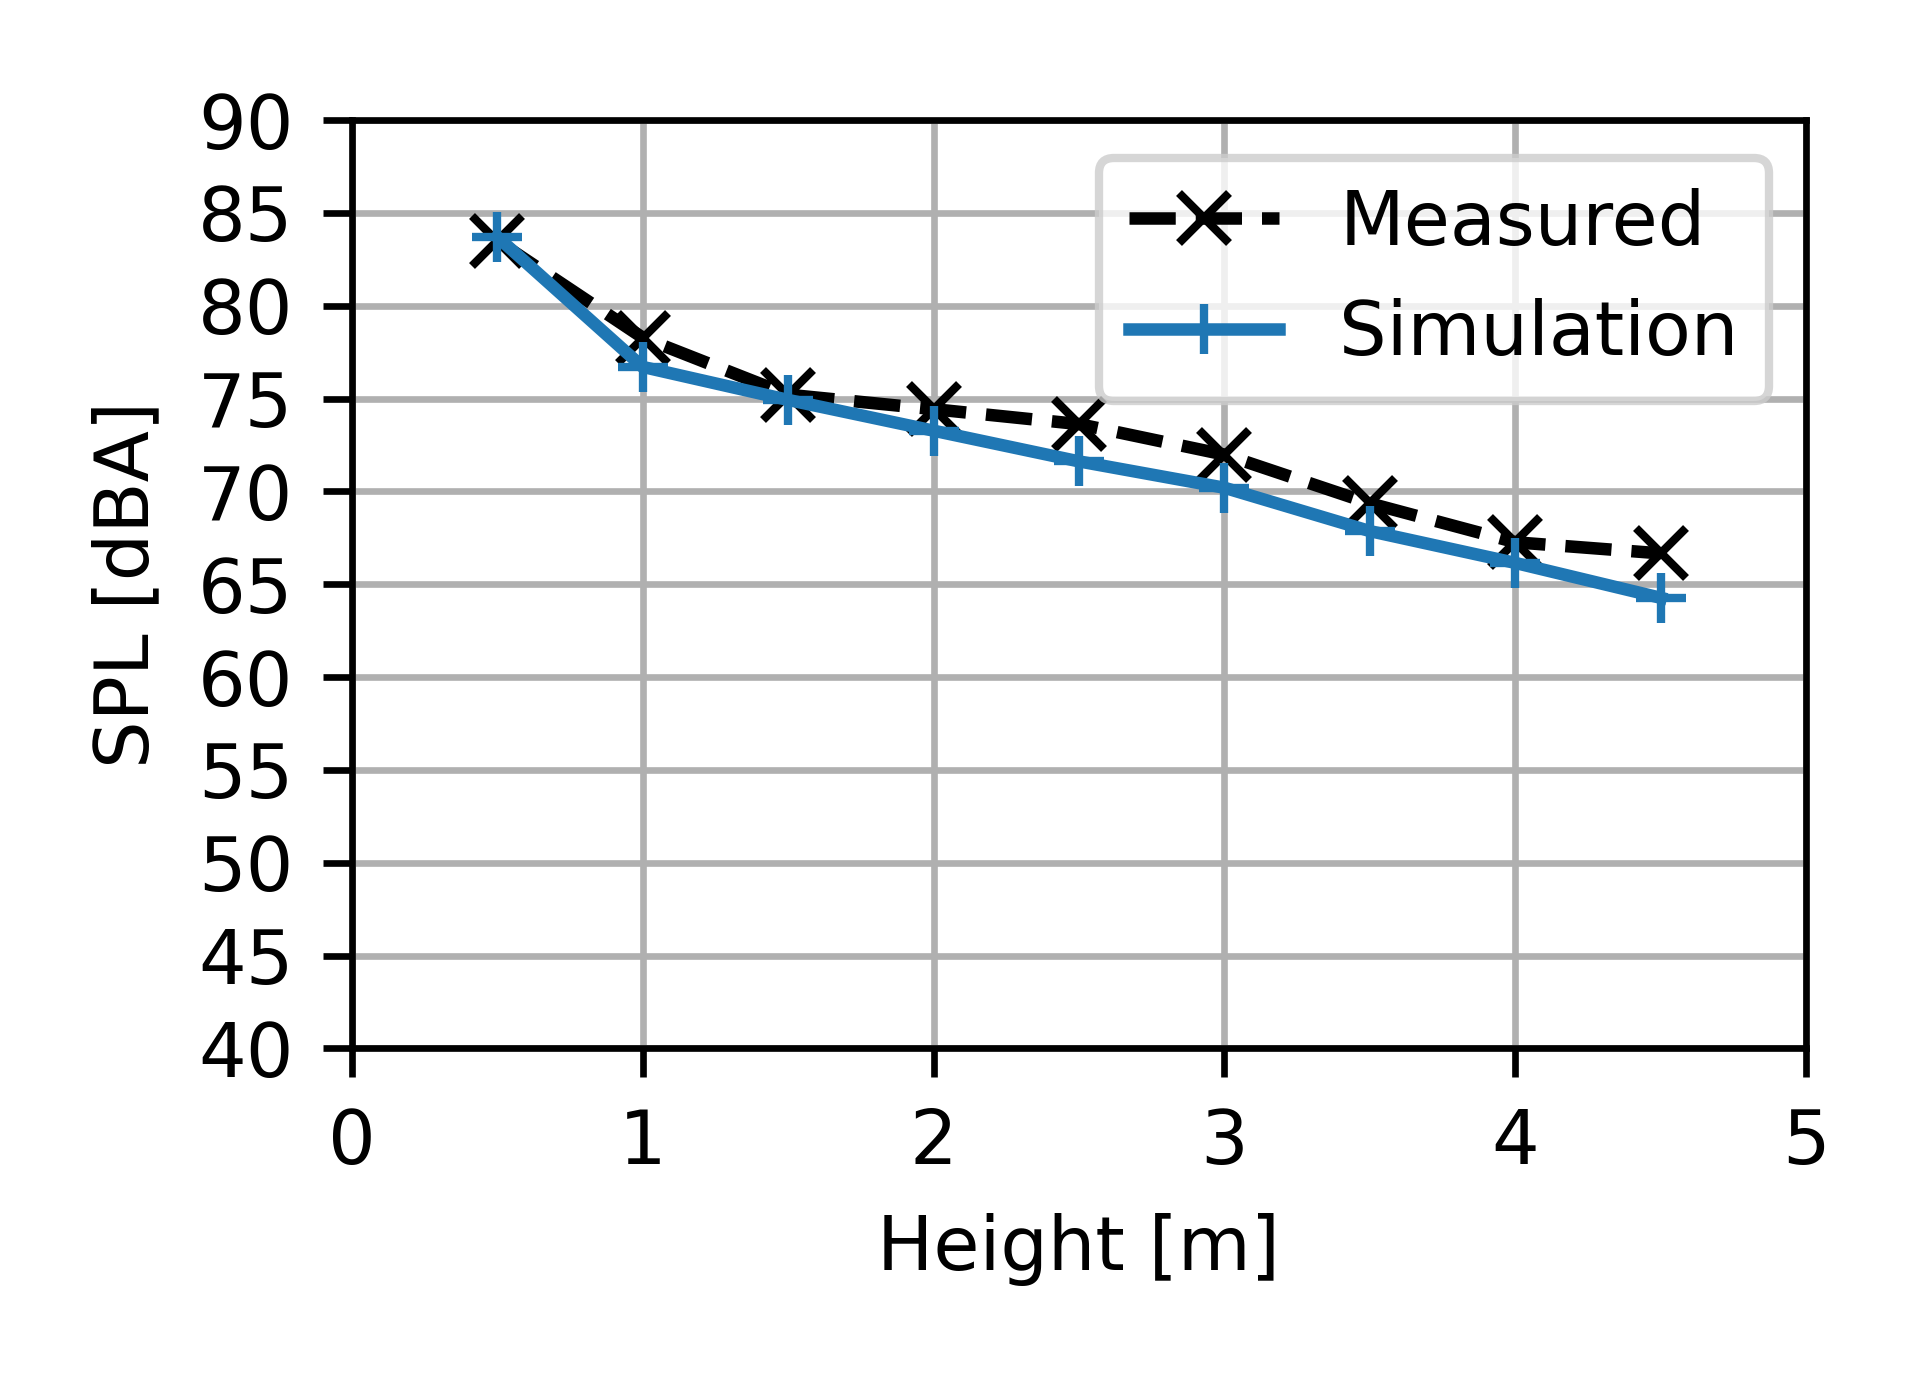
\includegraphics{fig/chap5/initial_model/third_octave_over_height/400_Hz.png}
		\caption{\SI{400}{\hertz}}
	\end{subfigure}
	\\
	\begin{subfigure}[b]{0.49\textwidth}
		\centering
		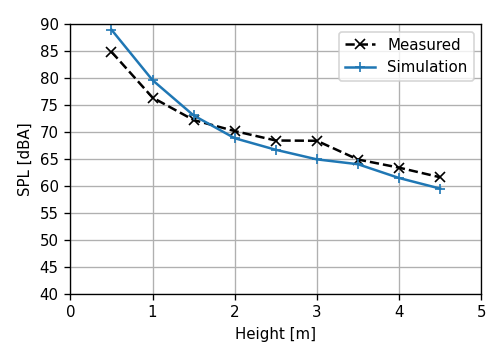
\includegraphics{fig/chap5/initial_model/third_octave_over_height/1250_Hz.png}
		\caption{\SI{1250}{\hertz}}
	\end{subfigure}
	\hfill
	\begin{subfigure}[b]{0.49\textwidth}
		\centering
		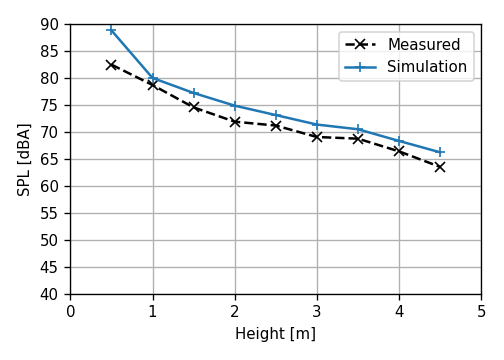
\includegraphics{fig/chap5/initial_model/third_octave_over_height/2000_Hz.png}
		\caption{\SI{2000}{\hertz}}
	\end{subfigure}
        \caption{Comparison between simulation (full line) and measurement (dashed line) over the height at measurement position a (\SI{10}{\centi\meter away from the carbody wall) for various one-third octave bands. A-weighted SPL in dBA ref \SI{20}{\micro\pascal}.}
	\label{fig:third_octave_over_height}
\end{figure}

In \cref{fig:third_octave_over_height}, the A-weighted sound pressure levels at measurement position a (\SI{10}{\centi\meter} away from vehicle) along the carbody height for various one-third octave bands are shown. The simulation result is compared with the measurement value at each microphone position. One can see that for \SI{125}{\hertz} and \SI{400}{\hertz}, the simulation fits the measured curves very well. A greater difference between the simulation and the measurement occurs for \SI{1250}{\hertz} and \SI{2000}{\hertz}, but the measured shape is still well approximated for both frequency bands. Other bands show similar results, and the model captures the measured sound pressure level trends well.

\begin{figure}%[H] avoid H and let latex place the floats
	\centering
	\begin{subfigure}[b]{0.49\textwidth}
		\centering
		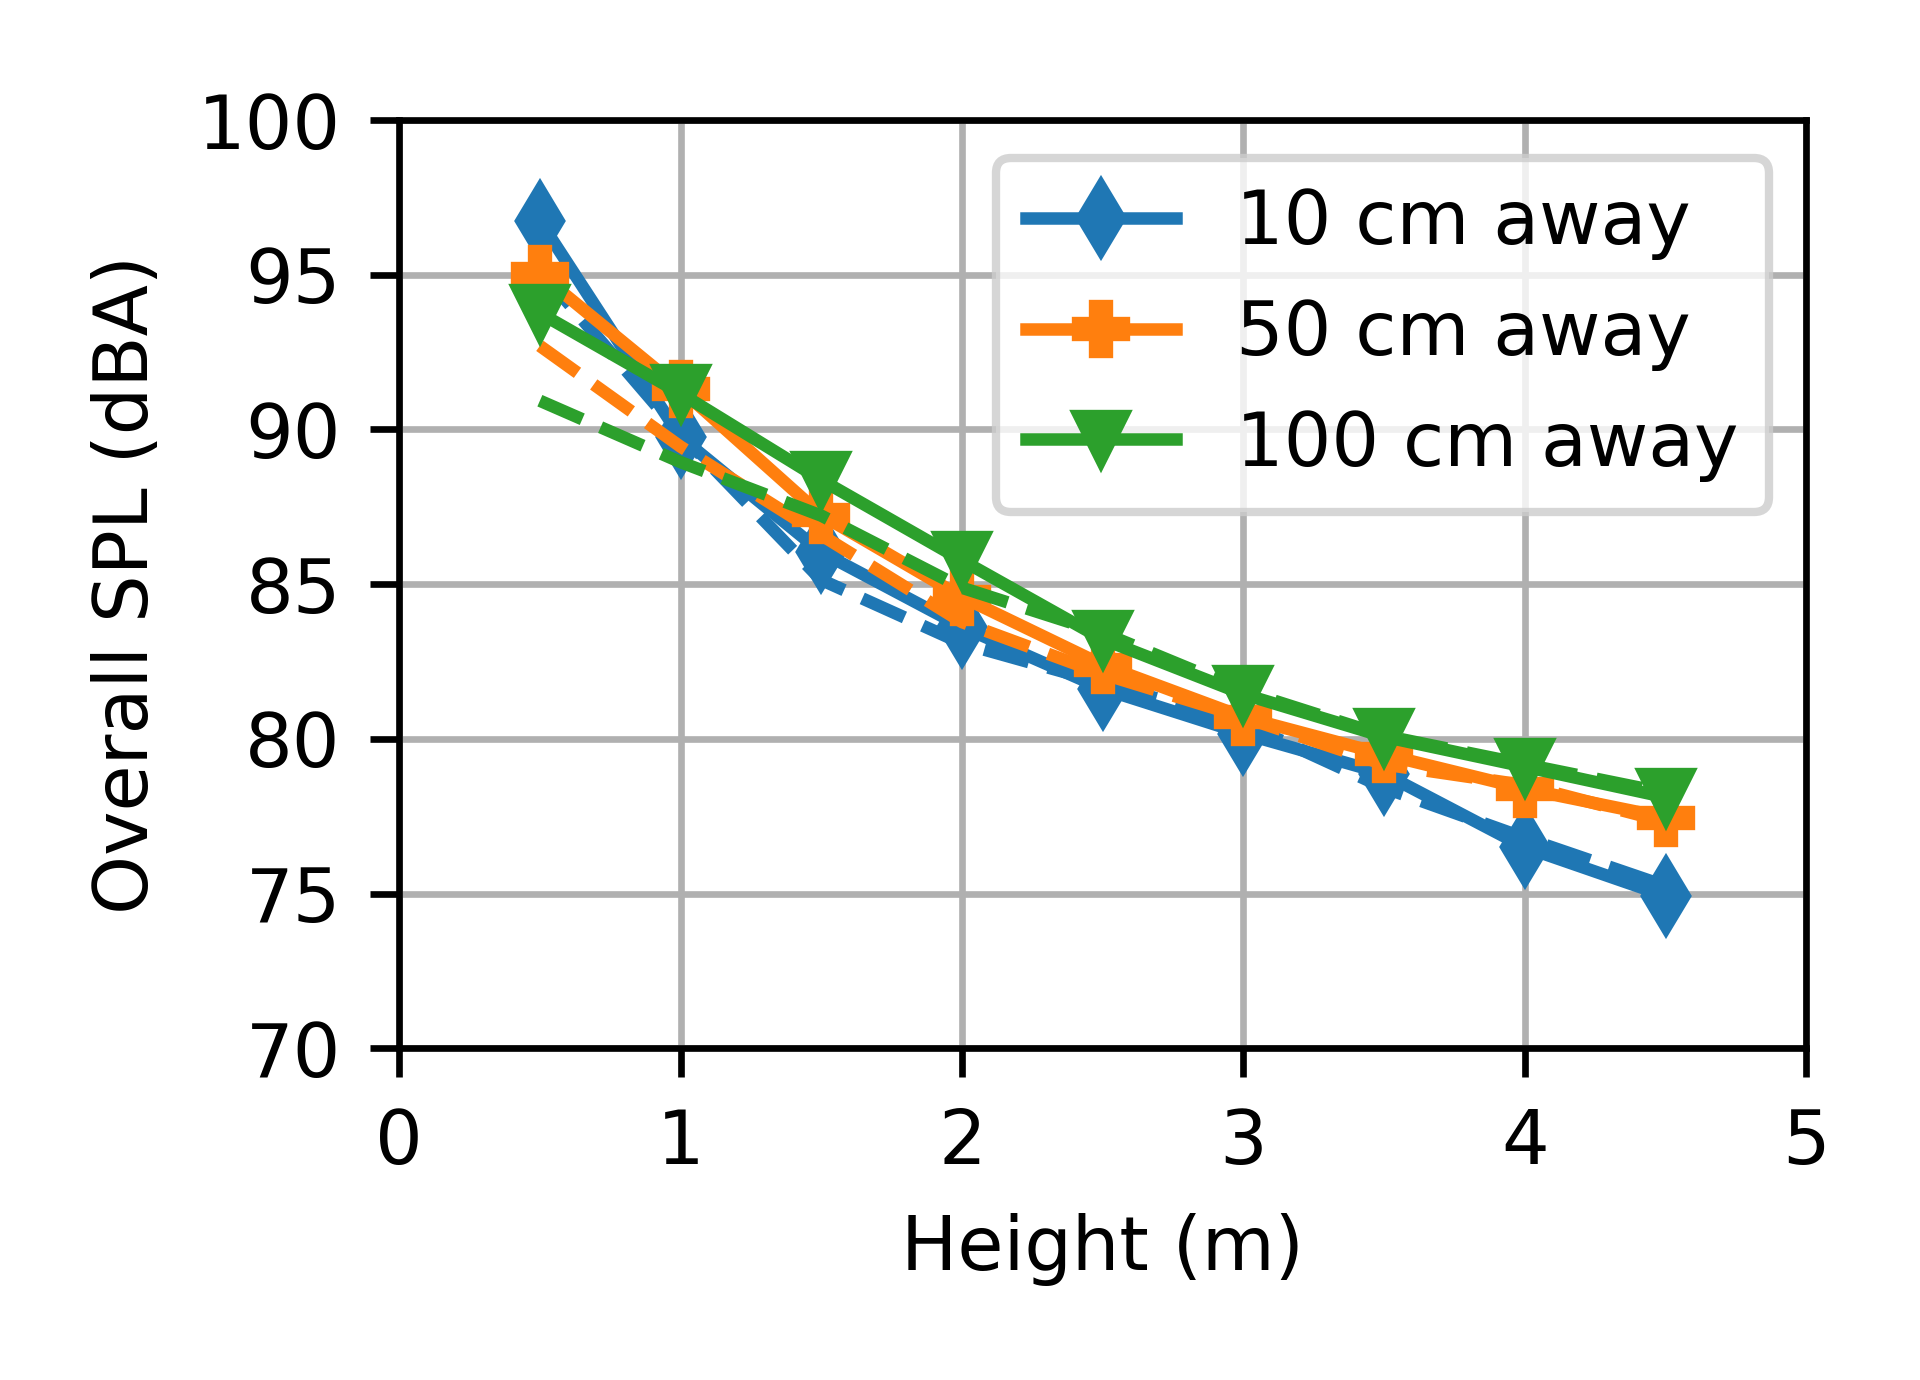
\includegraphics{fig/chap5/initial_model/overall_SPL/all_pos.png}
	\end{subfigure}
	\hfill
	\begin{subfigure}[b]{0.49\textwidth}
		\centering
		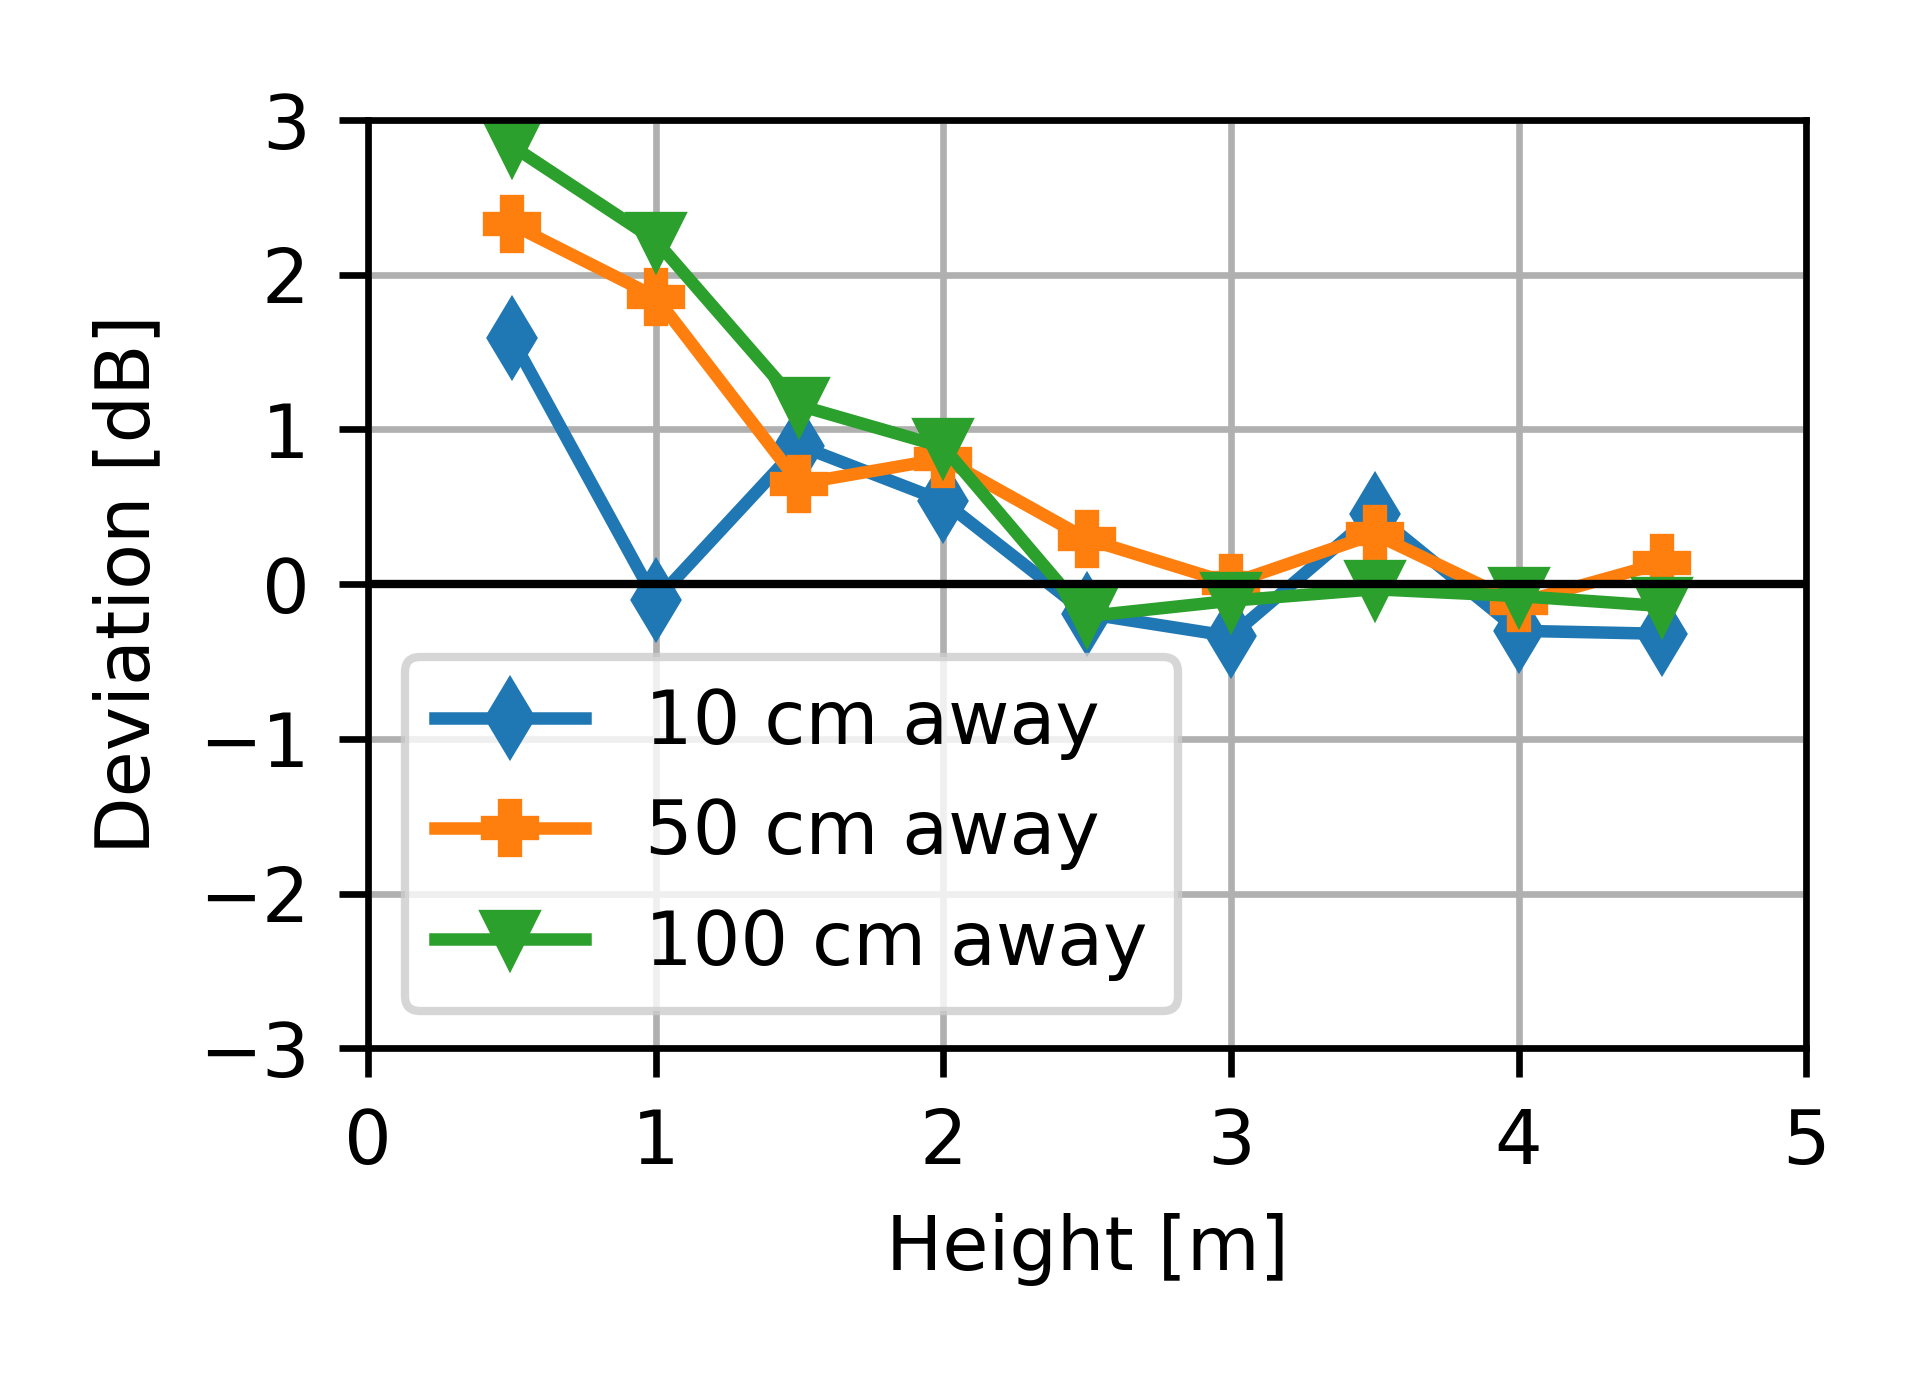
\includegraphics{fig/chap5/initial_model/overall_SPL/deviation.png}
	\end{subfigure}
	\caption{Comparison between simulation (full lines) and measurement (dashed lines) over the height at various measurement positions. Left: Overall SPL in dBA ref \SI{20}{\micro\pascal}; Right: Deviation between simulation and measurement results.}
	\label{fig:overall_SPL}
\end{figure}
% Put the figure and text in the same paragraph (no empty line)
% never use \noindent! Your paragraphs are indented!
The overall sound pressure level is a simple and direct parameter to quantify the sound level. 
For this comparison, the A-weighted sound pressure levels of each one-third octave band from \SIrange{100}{2000}{\hertz} are added up in decibels, yielding the \emph{overall SPL}. 
\Cref{fig:overall_SPL} shows the overall A-weighted sound pressure level at three different measurement positions and the deviation between the simulated and measured results. As can be seen from the results, the predictions of overall sound pressure levels at the three distances from the car body agree well with the measurement. For all three measurement positions, the maximum deviation between the simulation and measurement results occurs at \SI{0.5}{\meter}, which is at the height of the bogie. At these locations, the simulation results are \SI{1.5}{\decibel} to \SI{3}{\decibel} higher than the measured values. In general, the approximation improves with increasing height. In the area above \SI{2}{\meter}, the difference between the simulation and the measurement in terms of overall sound pressure is within \SI{1}{\decibel}.

\begin{figure}%[H]
	\centering
	\begin{subfigure}[b]{0.49\textwidth}
		\centering
		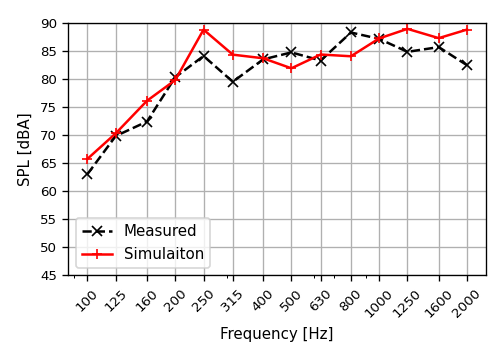
\includegraphics{fig/chap5/initial_model/freq_spectrum/pos_10cm_0pt5m.png}
		\caption{\SI{0.5}{\meter}}
	\end{subfigure}
	\hfill
	\begin{subfigure}[b]{0.49\textwidth}
		\centering
		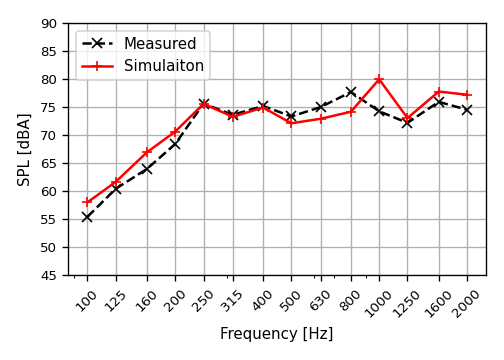
\includegraphics{fig/chap5/initial_model/freq_spectrum/pos_10cm_1pt5m.png}
		\caption{\SI{1.5}{\meter}}
	\end{subfigure}
%\end{figure}
%\begin{figure}[H] \ContinuedFloat
% try not to split floats, rather let latex make a float-page
	\begin{subfigure}[b]{0.49\textwidth}
		\centering
		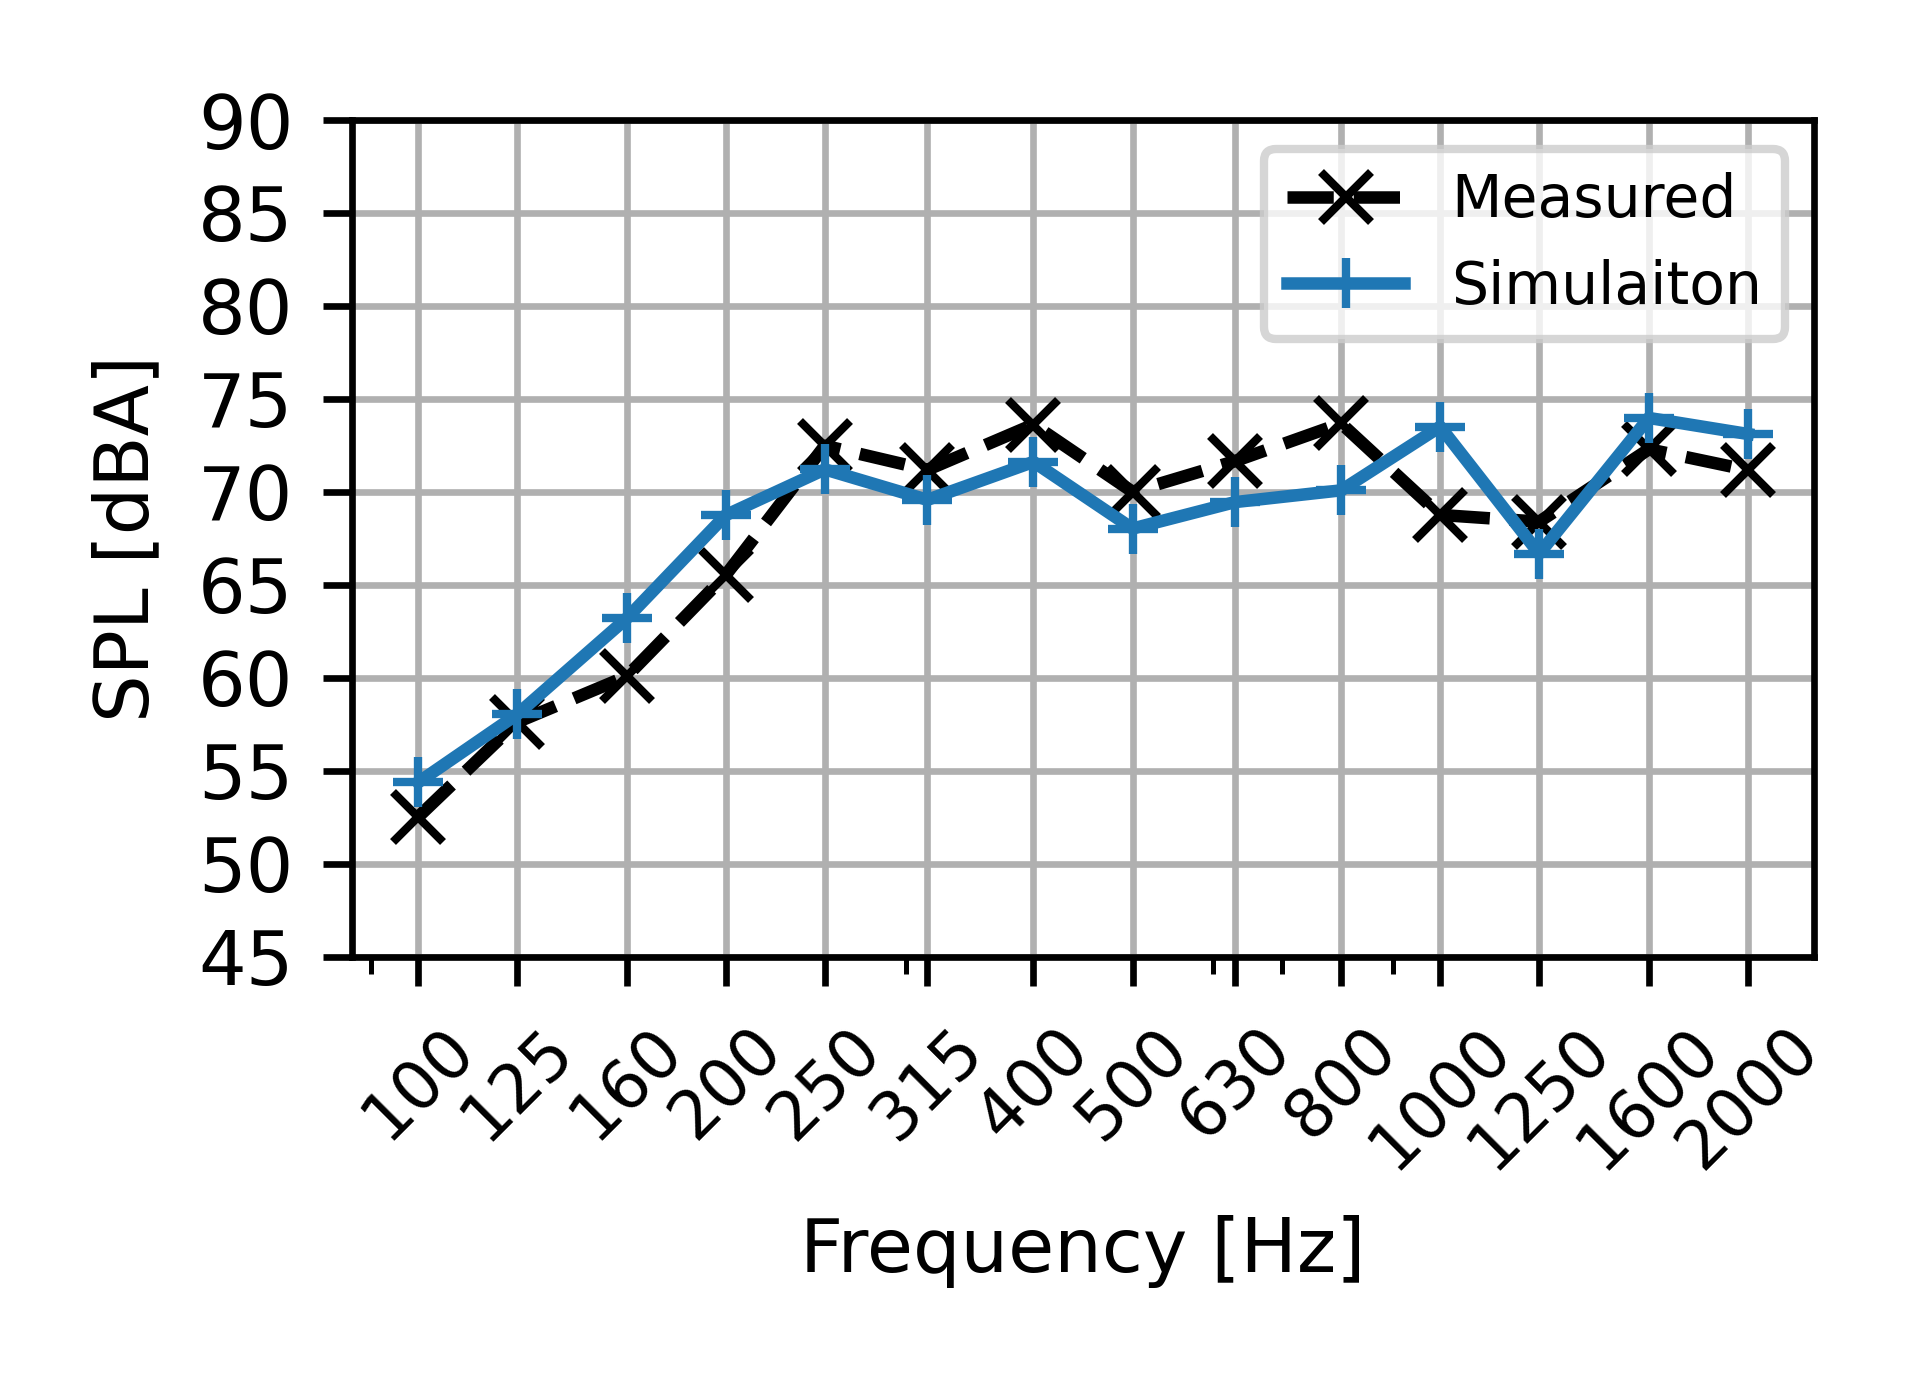
\includegraphics{fig/chap5/initial_model/freq_spectrum/pos_10cm_2pt5m.png}
		\caption{\SI{2.5}{\meter}}
	\end{subfigure}
	\hfill
	\begin{subfigure}[b]{0.49\textwidth}
		\centering
		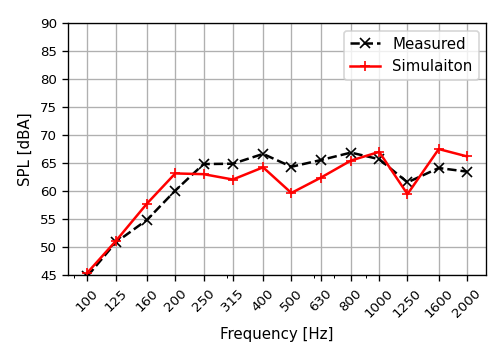
\includegraphics{fig/chap5/initial_model/freq_spectrum/pos_10cm_4pt5m.png}
		\caption{\SI{4.5}{\meter}}
	\end{subfigure}
	\caption{Comparison of the A-weighted SPL spectra between simulation (solid line) and measurement (dashed line) evaluated at measurement position a (\SI{10}{\centi\meter} away from the carbody wall) at various heights above ground.}
	\label{fig:freq_spectrum}
\end{figure}
%
\Cref{fig:freq_spectrum} shows the spectra of the A-weighted sound pressure level in one-third octave bands. The SPL spectra are evaluated at the measurement position a (\SI{10}{\centi\meter} away from the vehicle) at various heights. As can be seen from the results, the simulation fits the measured spectra well, the measured trend is well captured. Again, a larger deviation between the simulated and measured results occurs at \SI{0.5}{\meter} above ground and the approximation is getting better with increasing height.

In order to have an idea of the model accuracy of each 1/3-octave band, the mean relative error between the simulation result and the measurement for each 1/3-octave band over all 27 microphone positions will be computed. To compute the mean relative error, the sound pressure level is first converted back to linear scaling by
\begin{equation}
	p(\text{Pa}) = p_0 \cdot 10^{\frac{\text{SPL}}{20}} = 2\cdot10^{-5}\,\text{Pa} \cdot 10^{\frac{\text{SPL}}{20}}\text{.}
\end{equation}
The mean relative error (MRE) is then defined as
\begin{equation}
	\text{MRE}(p_{\text{measured}}, p_{\text{simulation}}) = \frac{1}{N} \sum_{i=0}^{N - 1} \frac{|p_{\text{simulation,}i} - p_{\text{measured,}i}|}{|p_{\text{measured,}i}|}\,.
\end{equation}
The mean relative error can also be converted to decibels using the relation
\begin{equation}
	\text{MRE(dB)} = 20\cdot\log_{10}(1 + \text{MRE})\,.
\end{equation}

\begin{figure}
	\centering
	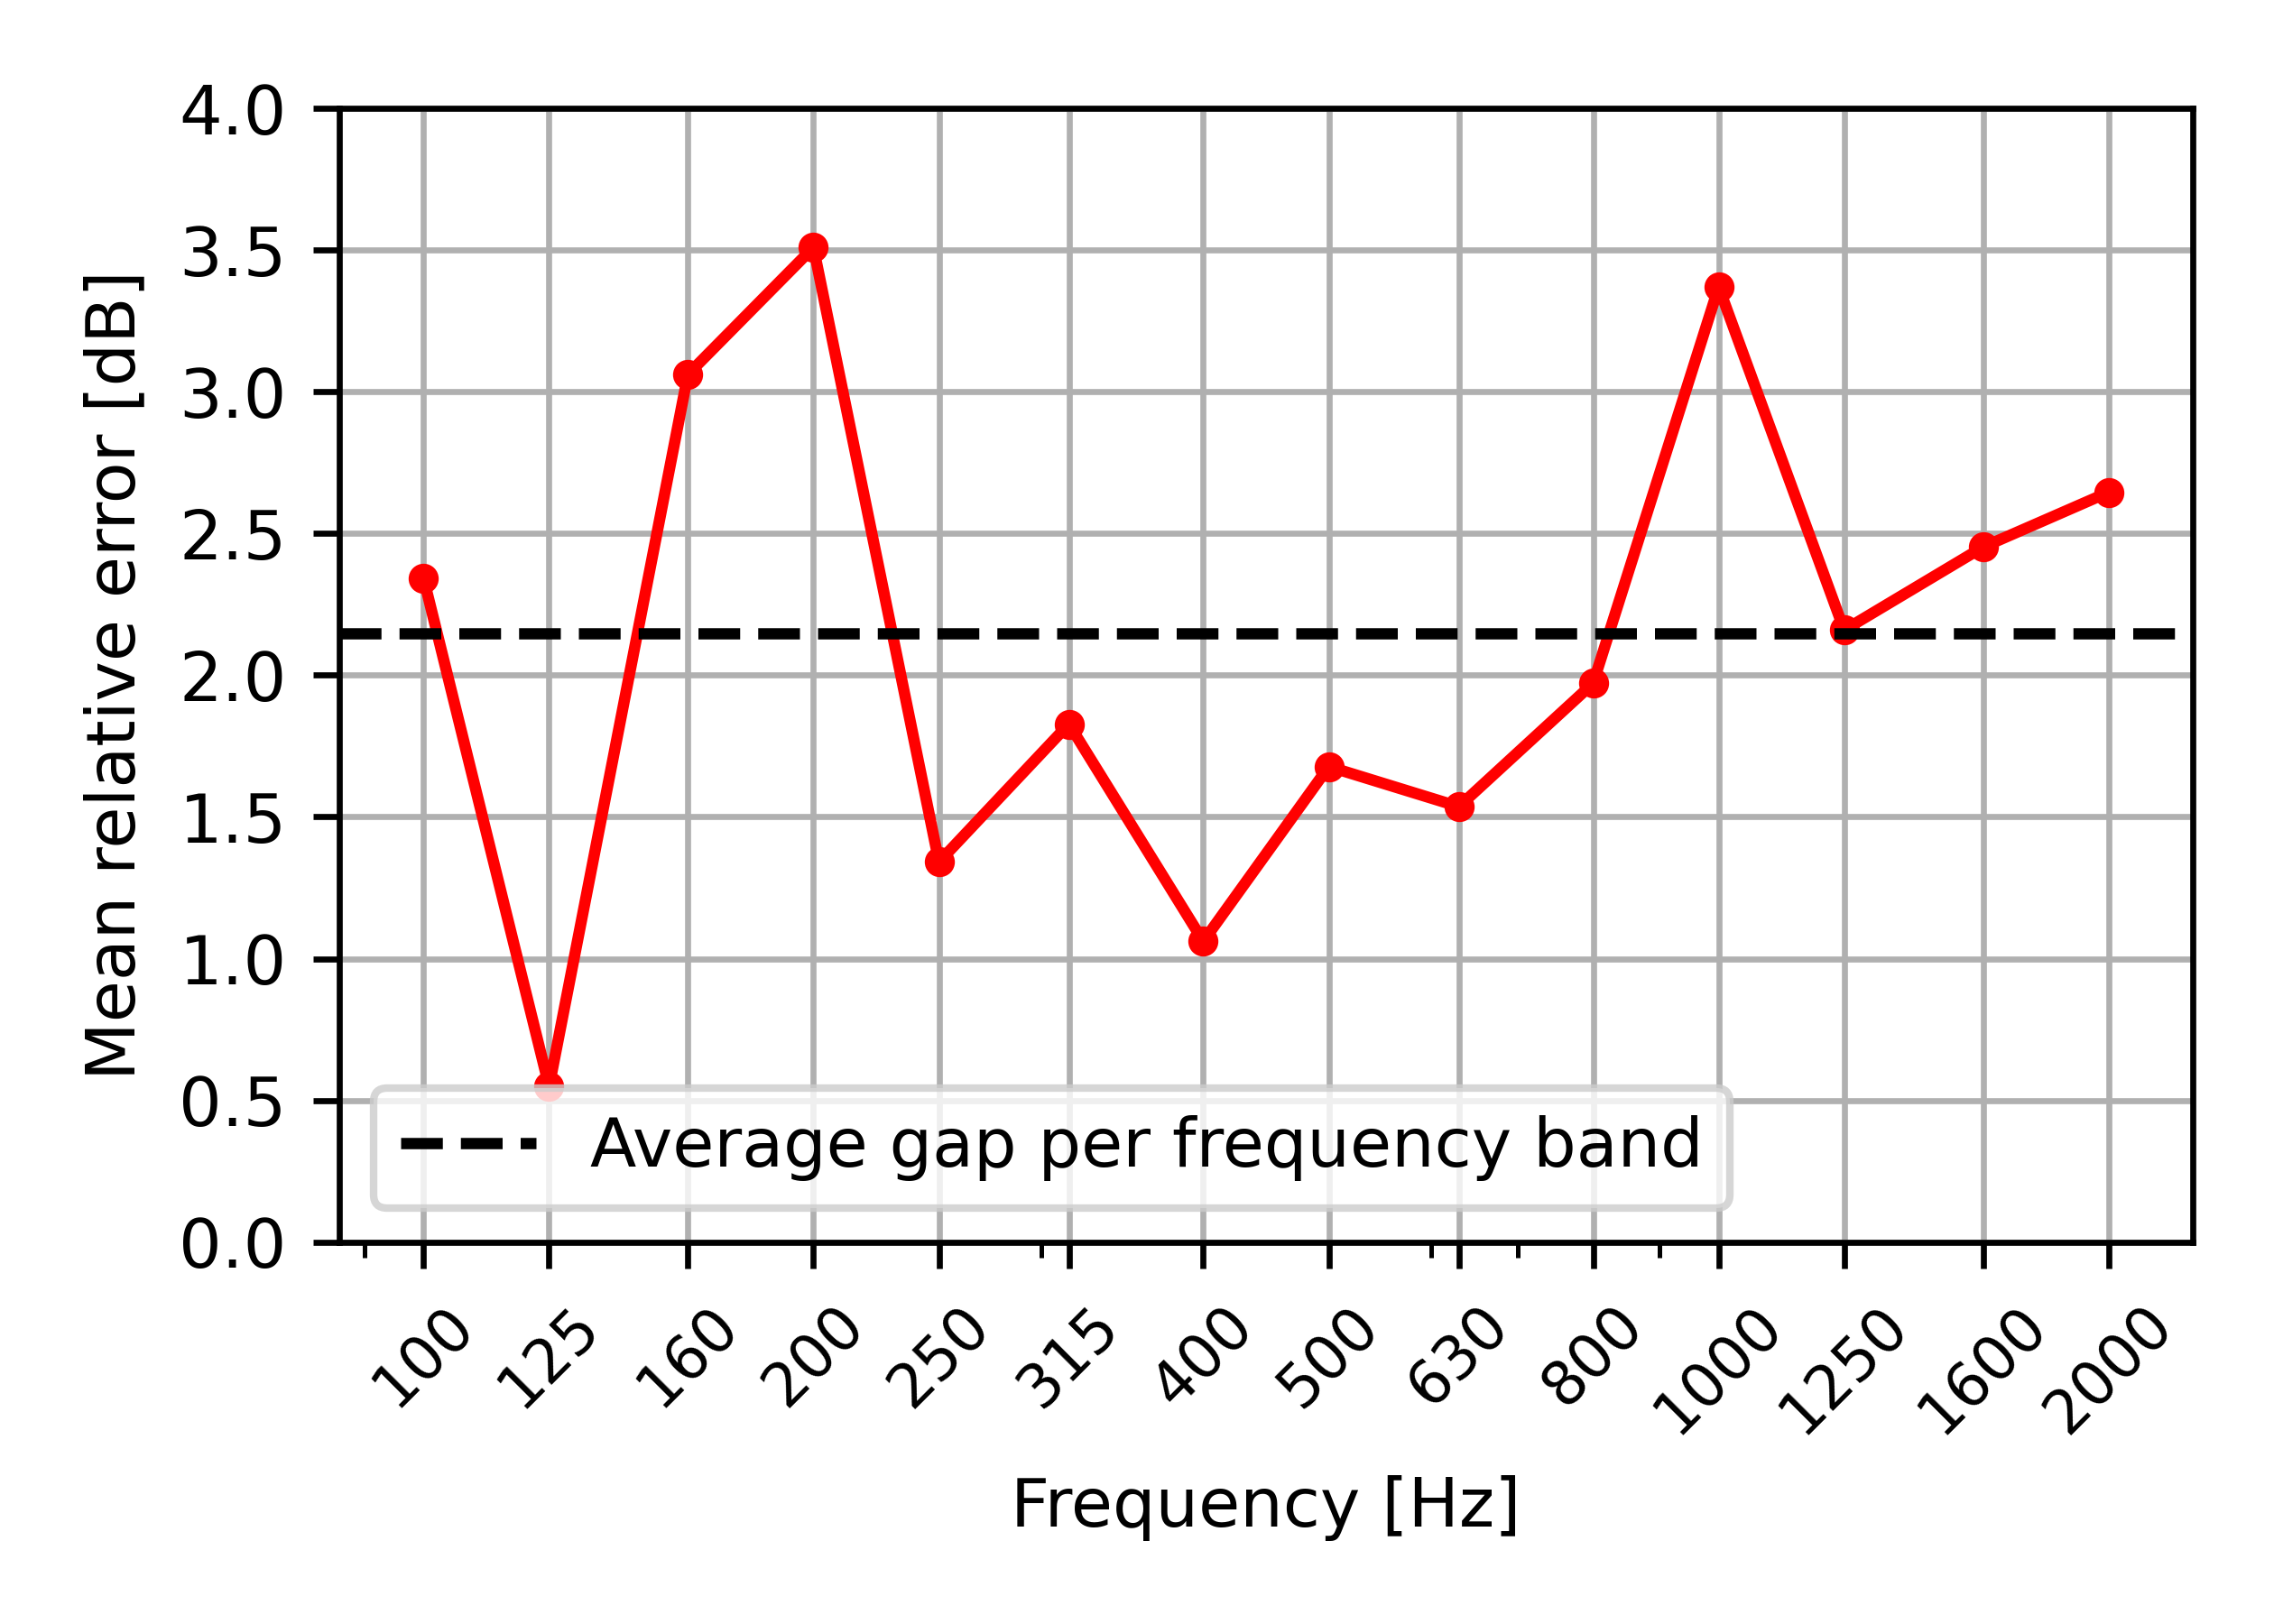
\includegraphics{fig/chap5/initial_model/freq_spectrum/average_gap.png}
	\caption{Mean relative error between simulation result and measurement for each 1/3-octave band over all 27 microphone positions.}
	\label{fig:gap_freq_spectrum}
\end{figure}

\begin{table}
	\centering
	\caption{Mean relative error of 1/3-octave frequency spectrum over all microphone positions.}
	\label{tab:MRE_spectra}
	\begin{tabular}{cccc}
		\begin{tabular}{cc}
			\toprule
			Frequency (Hz) & MRE (dB) \\
			\midrule
			100 & 2.34 \\
			125 & 0.55 \\
			160 & 3.06 \\
			200 & 3.51 \\
			250 & 1.34 \\
			315 & 1.82 \\
			400 & 1.06 \\
			\bottomrule
		\end{tabular} & 
		\begin{tabular}{cc}
			\toprule
			Frequency (Hz) & MRE (dB) \\
			\midrule
			500 & 1.67 \\
			630 & 1.53 \\
			800 & 1.97 \\
			1000 & 3.36 \\
			1250 & 2.15 \\
			1600 & 2.45 \\
			2000 & 2.65 \\
			\bottomrule
		\end{tabular}
	\end{tabular}
\end{table}


The mean relative error in terms of the sound pressure levels over all 27 microphone positions at each frequency band between the predictions and the measurements are shown in \cref{fig:gap_freq_spectrum} and in \cref{tab:MRE_spectra}. As can be seen from the results, the best approximation occurs for the \SI{125}{\hertz} band which has the smallest mean relative error among all 1/3 octave bands. Three frequency bands (\SI{160}{\hertz}, \SI{200}{\hertz} and \SI{1000}{\hertz}) have an error over \SI{3}{\decibel}, and the maximum error is limited by \SI{3.5}{\decibel}. Good approximation has also been shown for the frequency bands from \SIrange{250}{800}{\hertz}, for which the mean relative errors are within \SI{2}{\decibel}. The average gap per frequency band is obtained by averaging the mean relative error spectrum over all 14 one-third octave bands. Following the same idea, the mean relative error in terms of overall sound pressure levels will also be used as a metric for model accuracy.

The average gap per frequency band and the mean relative error of overall sound pressure levels over all microphone positions are shown in \cref{tab:average_gap}.
The average difference per frequency band is \SI{2.14}{\decibel} and the mean relative error of the overall sound pressure level is \SI{0.73}{\decibel}. From these results, it can be concluded that the finite element model is able to predict the sound transmission from the train underfloor with adequate accuracy.

\begin{table}%[H] never break a paragraph by a float within it.
	\centering
	\caption{Average gap per frequency band and mean relative error of overall SPL of the initial model.}
	\begin{tabular}{cc}
		\toprule
		Average gap per  frequency band (dB) & Mean relative error of overall SPL (dB) \\
		\midrule
		%$2.14\pm1$  & $0.73\pm0.86$
		2.14 & 0.73 \\
		\bottomrule
	\end{tabular}
	\label{tab:average_gap}
\end{table}


\section{Effect of geometric variation}

In this section, the results obtained by the variation analysis of underfloor geometry are shown. The geometrical models are illustrated and explained in \cref{section:variation_geometry}.

\begin{figure}
	\centering
	\begin{subfigure}[b]{0.49\textwidth}
		\centering
		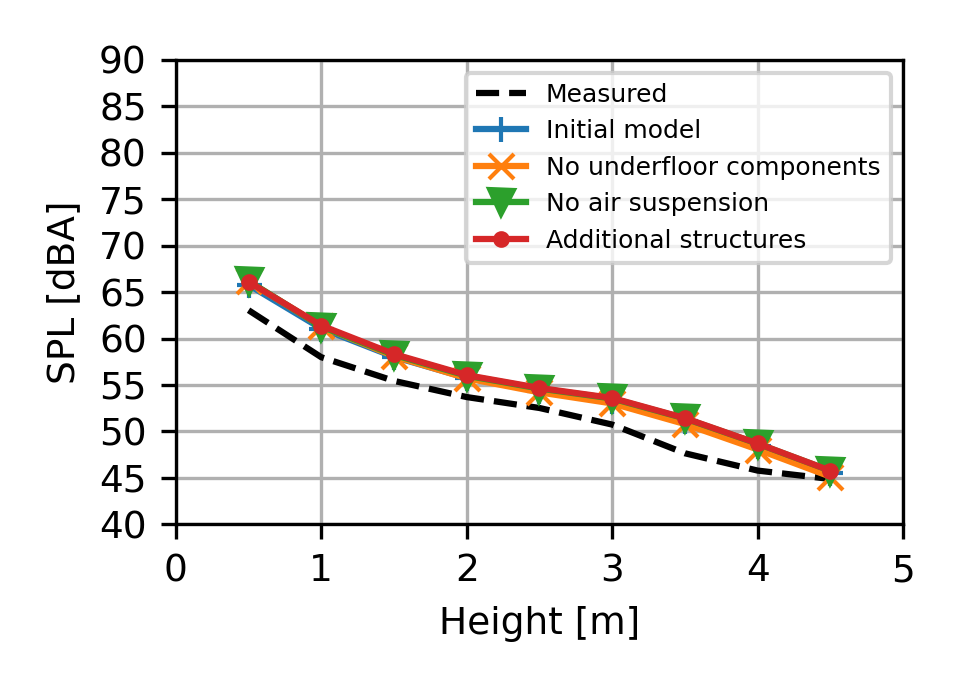
\includegraphics{fig/chap5/geometry_variation/third_octave_over_height/100_Hz.png}
		\caption{\SI{100}{\hertz}}
	\end{subfigure}
	\hfill
	\begin{subfigure}[b]{0.49\textwidth}
		\centering
		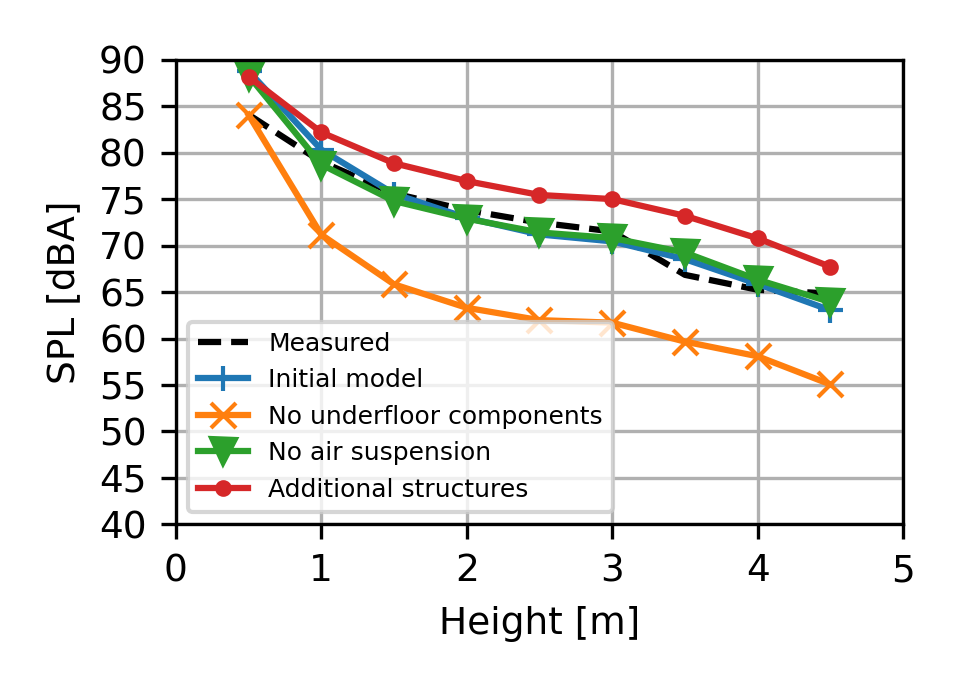
\includegraphics{fig/chap5/geometry_variation/third_octave_over_height/250_Hz.png}
		\caption{\SI{250}{\hertz}}
	\end{subfigure}
	\\
	\begin{subfigure}[b]{0.49\textwidth}
		\centering
		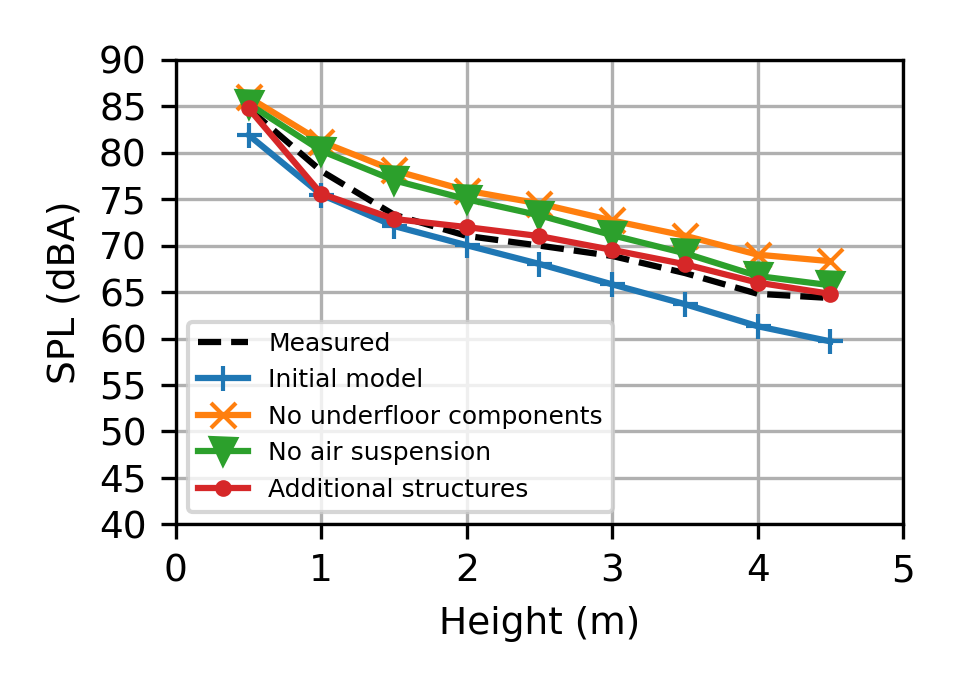
\includegraphics{fig/chap5/geometry_variation/third_octave_over_height/500_Hz.png}
		\caption{\SI{500}{\hertz}}
	\end{subfigure}
	\hfill
	\begin{subfigure}[b]{0.49\textwidth}
		\centering
		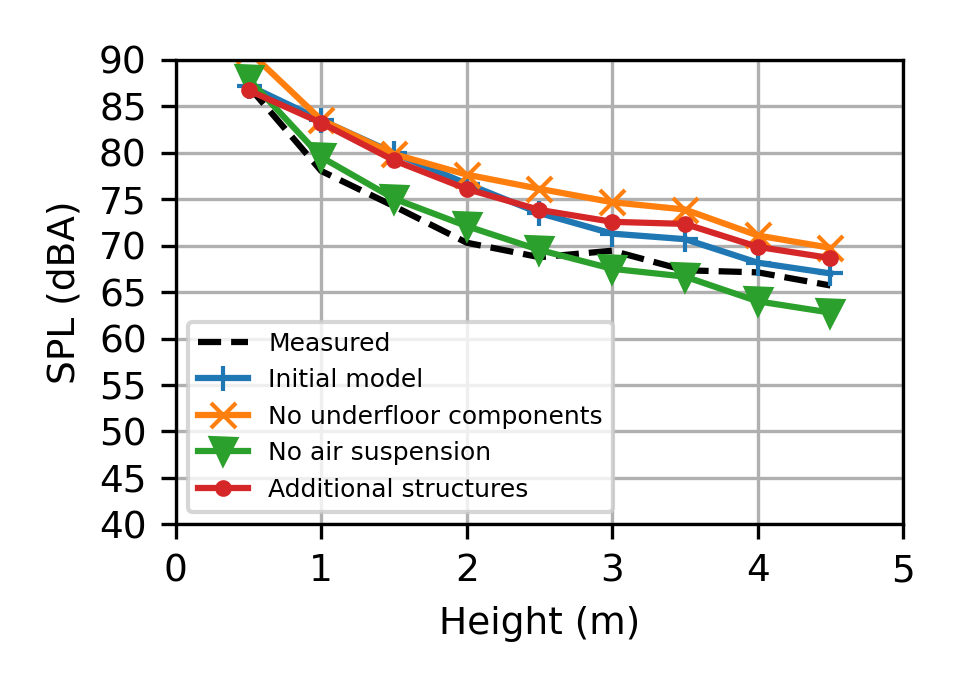
\includegraphics{fig/chap5/geometry_variation/third_octave_over_height/1000_Hz.png}
		\caption{\SI{1000}{\hertz}}
	\end{subfigure}
	\caption{Sound pressure level over the height at measurement position a, comparison between different geometrical models (solid lines) and the measurement (dashed lines). SPL in dBA ref \SI{20}{\micro\pascal}.}
	\label{fig:third_octave_over_height_geometry_variation}
\end{figure}

\Cref{fig:third_octave_over_height_geometry_variation} shows the A-weighted sound pressure level at measurement position a (\SI{10}{\centi\meter} away from vehicle) for different geometry variations in example one-third octave bands. As can be seen from the results, there is almost no difference between the different models at the lowest frequency band (\SI{100}{\hertz}). This may be because the wavelength (about \SI{3.43}{\meter} for \SI{100}{\hertz}) is much larger than the characteristic physical dimensions of the geometry. At this frequency, all four models overestimate the sound pressure level by about \SI{3}{\decibel} but are still able to capture the measured curve shape well. A large deviation between the models is found at \SI{250}{\hertz}, where the model without underfloor components underestimates the measurement result and the model with additional structures tends to overestimate them. The initial model and the model without air suspension show very good agreement with the measurement data. For \SI{500}{\hertz} and \SI{1000}{\hertz}, the model with additional structures and the model without air suspension agree well with the measurement data. In general, all models show similar shapes as the measurement curves, the differences in terms of sound pressure level between the four models are within \SI{10}{\decibel}. Very similar results are also observed for other frequency bands.

\begin{figure}
	\centering
	\begin{subfigure}[b]{\textwidth}
		\centering
		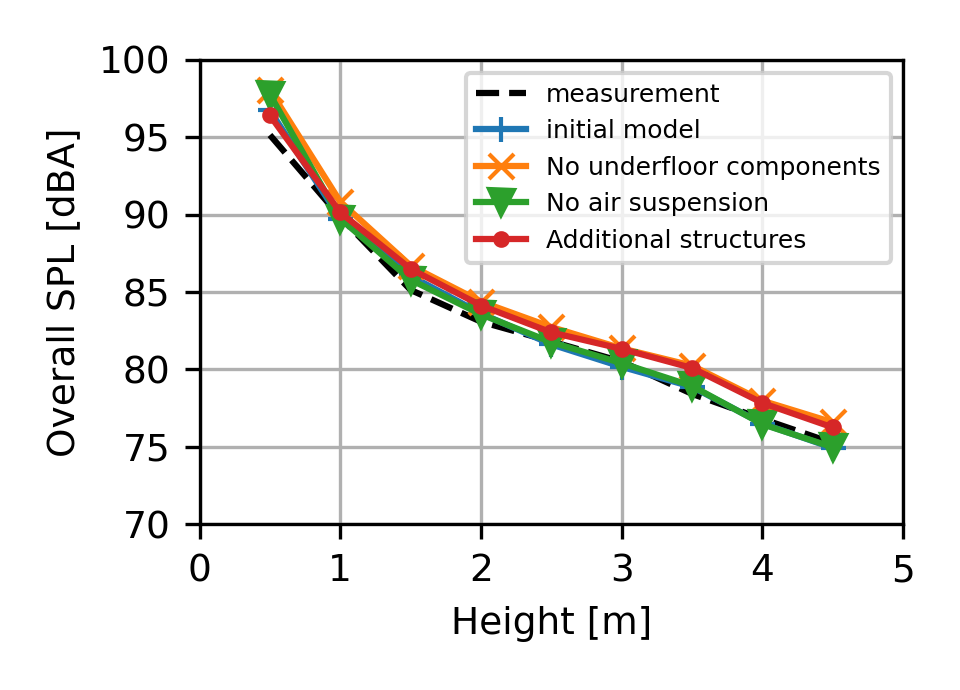
\includegraphics{fig/chap5/geometry_variation/overall_SPL/pos_a.png}
		\hfill
		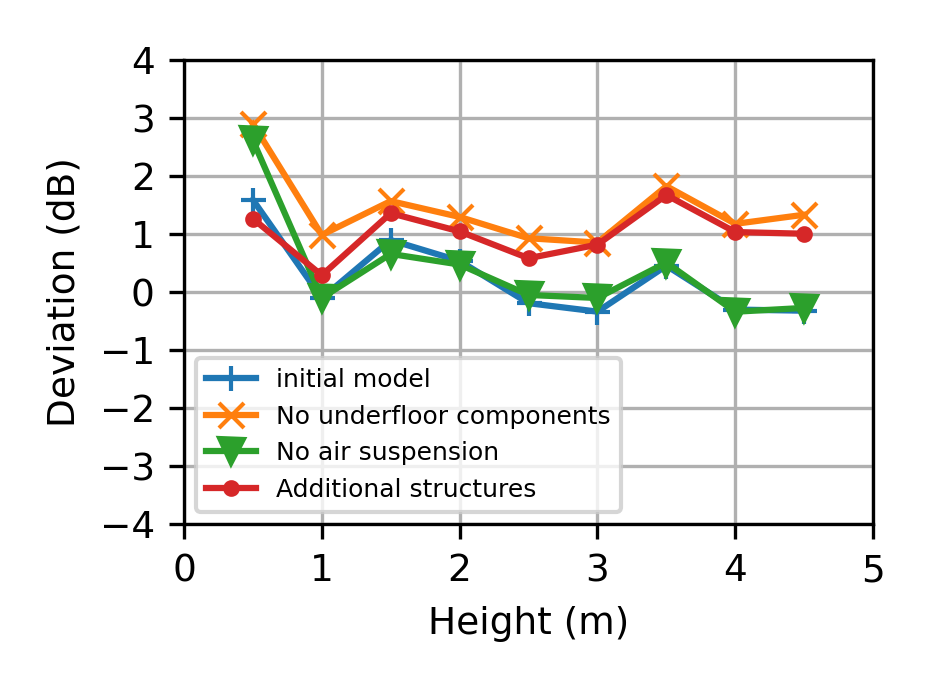
\includegraphics{fig/chap5/geometry_variation/overall_SPL/pos_a_deviation.png}
		\caption{\SI{10}{\centi\meter} away from carbody.}
	\end{subfigure}
	\\
	\begin{subfigure}[b]{\textwidth}
		\centering
		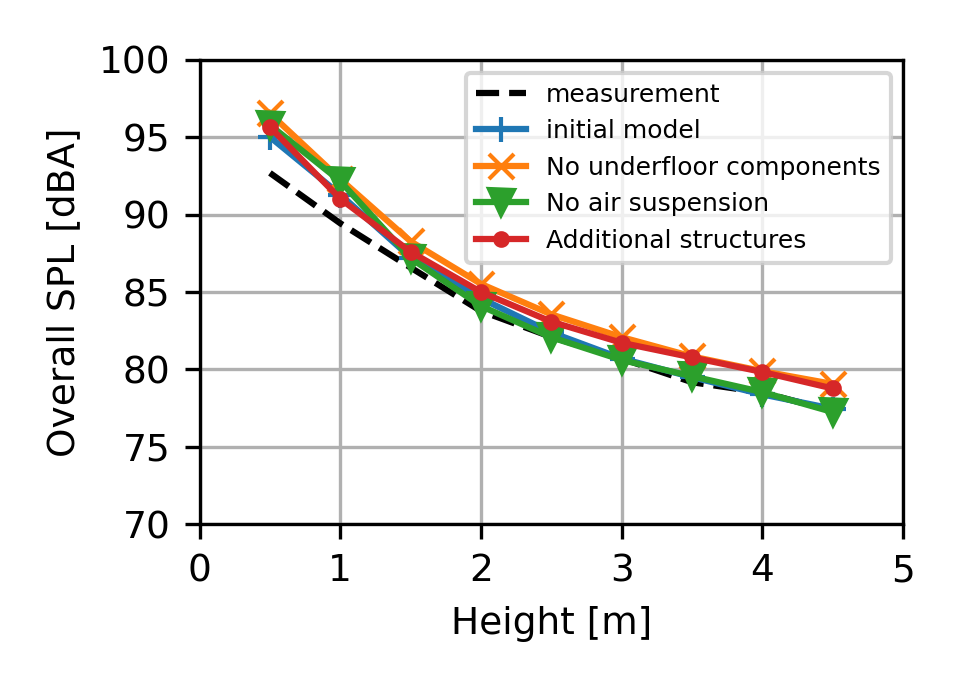
\includegraphics{fig/chap5/geometry_variation/overall_SPL/pos_f.png}
		\hfill
		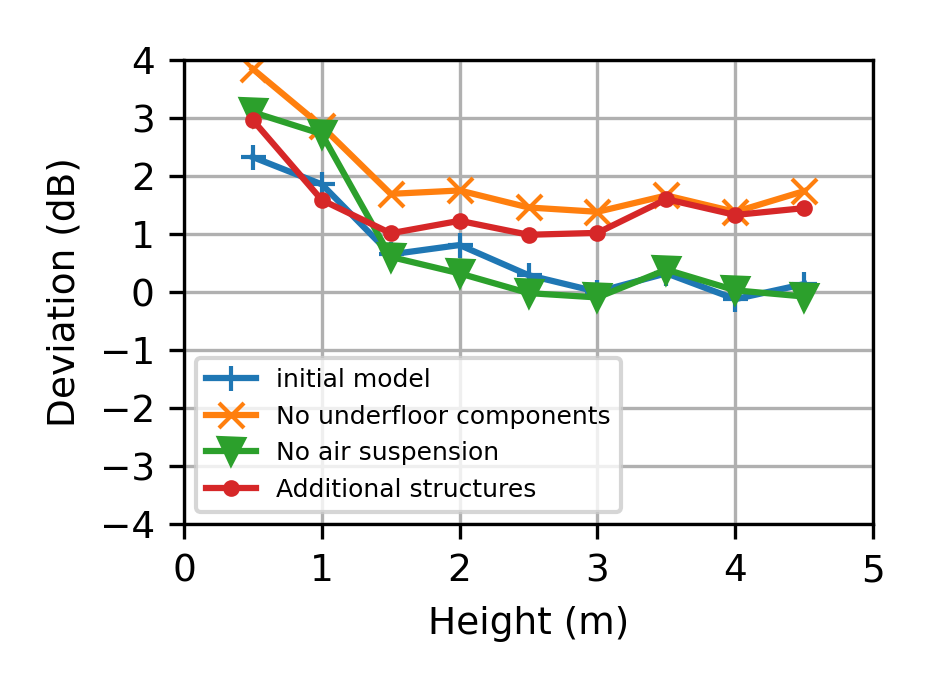
\includegraphics{fig/chap5/geometry_variation/overall_SPL/pos_f_deviation.png}
		\caption{\SI{50}{\centi\meter} away from carbody}
	\end{subfigure}
	\caption{Comparison between simulation (solid lines) and measurement (dashed lines) over the height at various measurement positions for different geometrical models. Left: Overall SPL in dBA ref \SI{20}{\micro\pascal}. Right: Deviation between simulation and measurement results.}
	\label{fig:overall_SPL_geometry}
\end{figure}

\Cref{fig:overall_SPL_geometry} shows the distribution of  A-weighted overall sound pressure levels at different distances from the carbody for different geometrical models.
As can be seen from the figures, all four models show similar results in the lower area (up to \SI{2}{\meter} height), the deviation between the models starts to grow with increasing height. Comparing the initial model and the model without air suspension, the model without air suspension shows a greater overestimation of the overall SPL than the initial model at the height of the bogie (\SI{0.5}{\meter}). Up from \SI{1.5}{\meter} height, both models show very good agreement with the measurement results and there is almost no difference between both models. One can also see that without including any underfloor components in the model, the overall SPL is overestimated at each measurement location due to a lack of shielding of the acoustic wave by the underfloor components. The difference between the initial model and the model without underfloor components is about \SIrange{1}{1.5}{\decibel}, depending on the measurement locations. The model with additional underfloor structures shows a similar result as the initial model at \SI{0.5}{\meter} height, but in the higher region (up from \SI{1.5}{\meter}), the result converges to that of the model without underfloor components.

\begin{figure}
	\centering
	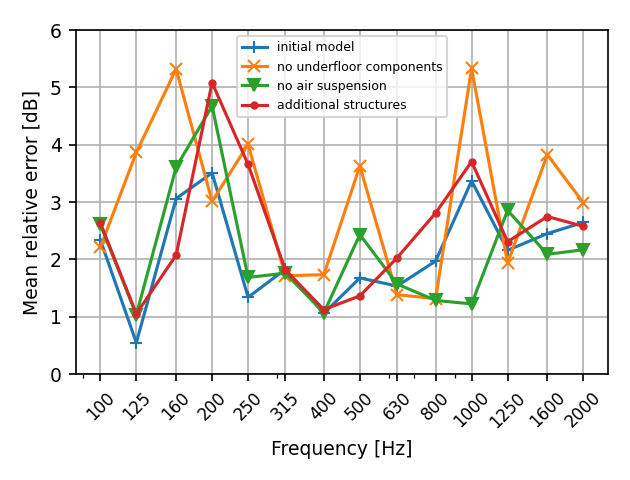
\includegraphics[width=0.7\linewidth]{fig/chap5/geometry_variation/freq_spectrum/average_gap.png}
	\caption{Mean relative error of 1/3-octave frequency for different geometry variations.}
	\label{fig:gap_freq_spectrum_geometry}
\end{figure}

\Cref{fig:gap_freq_spectrum_geometry} shows the mean relative error spectra for the four geometrical models over all 27 microphone locations. The spectrum of the initial model has also been shown in \cref{fig:gap_freq_spectrum}. As can be seen from the figure, all three geometry variations show greater maximum error than the initial model. For a large part of the frequency bands, the model without underfloor components has the greatest deviation among the models. At frequency band \SI{100}{\hertz}, \SI{315}{\hertz}, \SI{400}{\hertz}, \SI{630}{\hertz} and \SI{2000}{\hertz}, the difference in terms of the mean relative error among the models is small and limited by \SI{1}{\decibel}. The initial model and the model without air suspension share similar results, but at frequency band \SI{800}{\hertz}, \SI{1000}{\hertz}, \SI{1600}{\hertz} and \SI{2000}{\hertz}, the latter model shows better approximation than the former.

\begin{table}
	\centering
	\caption{Average gap per frequency band and mean relative error in overall SPL for different geometry variations.}
	\label{tab:geometry_variation_MRE}
	\begin{tabular}{ccc}
		\toprule
		Geometry name              & Average gap per frequency band (dB) & MRE overall SPL (dB) \\
		\midrule
		No underfloor components   & $3.12$                       & $1.78$        \\
		No air suspension          & $2.21$                       & $0.85$        \\
		Initial model              & $2.34$                       & $0.73$        \\
		With additional structures & $2.57$                       & $1.30$ \\
		\bottomrule  
	\end{tabular}
\end{table}

In order to quantify the difference between the geometry variations, the average gap per frequency band and the mean relative error in terms of overall SPL are computed and shown in \cref{tab:geometry_variation_MRE}. The table is ordered by the complexity of the modeled geometry. As can be seen from results, the simplest model, namely the model without any underfloor components, shows the greatest average gap per frequency band as well as the largest mean relative error in terms of the overall sound pressure level. Both errors are reduced by almost \SI{1}{\decibel} by including the most essential underfloor components (bogie and wheel) into the model. Taking the air suspension into account leads to a better approximation for the overall SPL, but a slightly increased average gap per frequency band, which may be due to the assumption of a sound hard boundary at the air suspension interface. Surprisingly, the model with additional structures shows a greater deviation in both metrics compared to the initial model. It was expected that including more underfloor details will also lead to a better approximation of the measurement. It can be concluded from the results shown in this section that the number of modeled underfloor components affect the prediction accuracy of the finite element model. To achieve better approximation of the measurement data, the bogie and the wheel at a minimum should be taken into the geometrical model. Without modeling the underfloor components, the predicted overall SPL is about \SI{1}{\decibel} higher compared to the prediction using model with underfloor components.

\section{Effect of ground absorption}

In this section, the simulation results obtained by the variation analysis of the surface impedance are shown. Note that all variation models have the same normal incident absorption coefficient and only differ in their impedance phase angle. Since the absorption data used for the simulation is fictive, the results are not compared to the validation measurement but to the initial model with fully reflective ground.

\begin{figure}
	\centering
	\begin{subfigure}[b]{\textwidth}
		\centering
		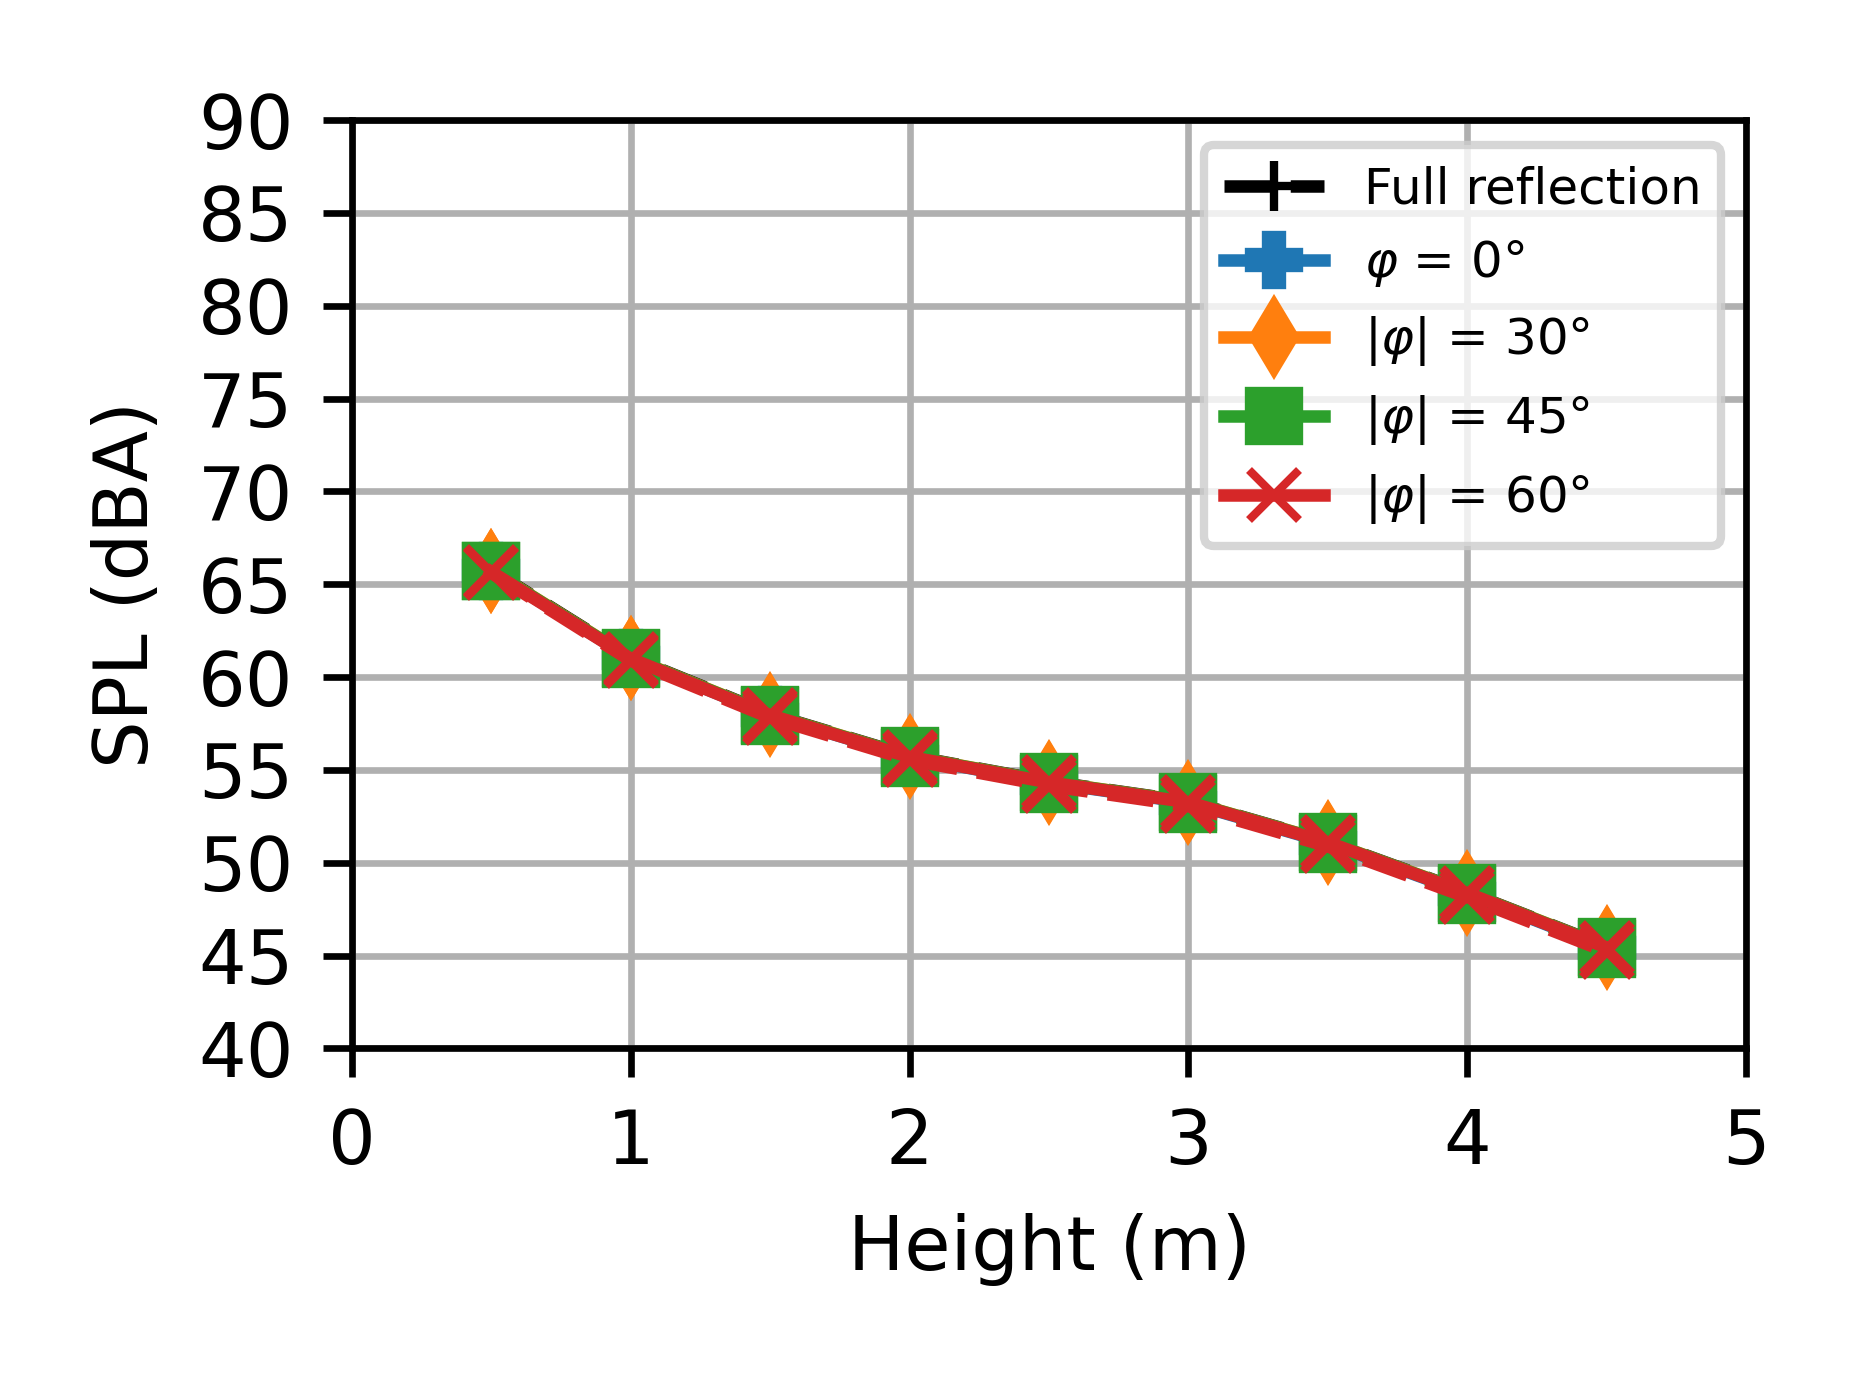
\includegraphics{fig/chap5/impedance/third_octave/SPL_100_Hz.png}
		\hfill
		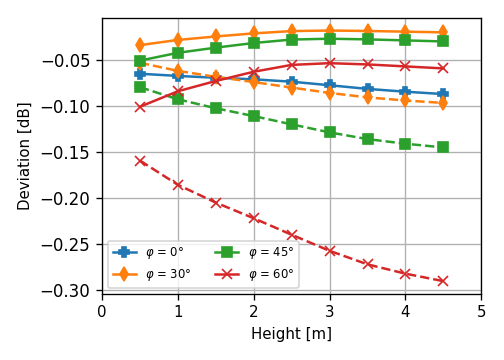
\includegraphics{fig/chap5/impedance/third_octave/deviation_100_Hz.png}
		\caption{\SI{100}{\hertz}}
	\end{subfigure}
	\\
	\begin{subfigure}[b]{\textwidth}
		\centering
		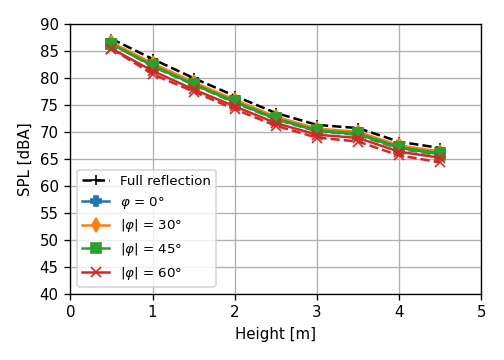
\includegraphics{fig/chap5/impedance/third_octave/SPL_1000_Hz.png}
		\hfill
		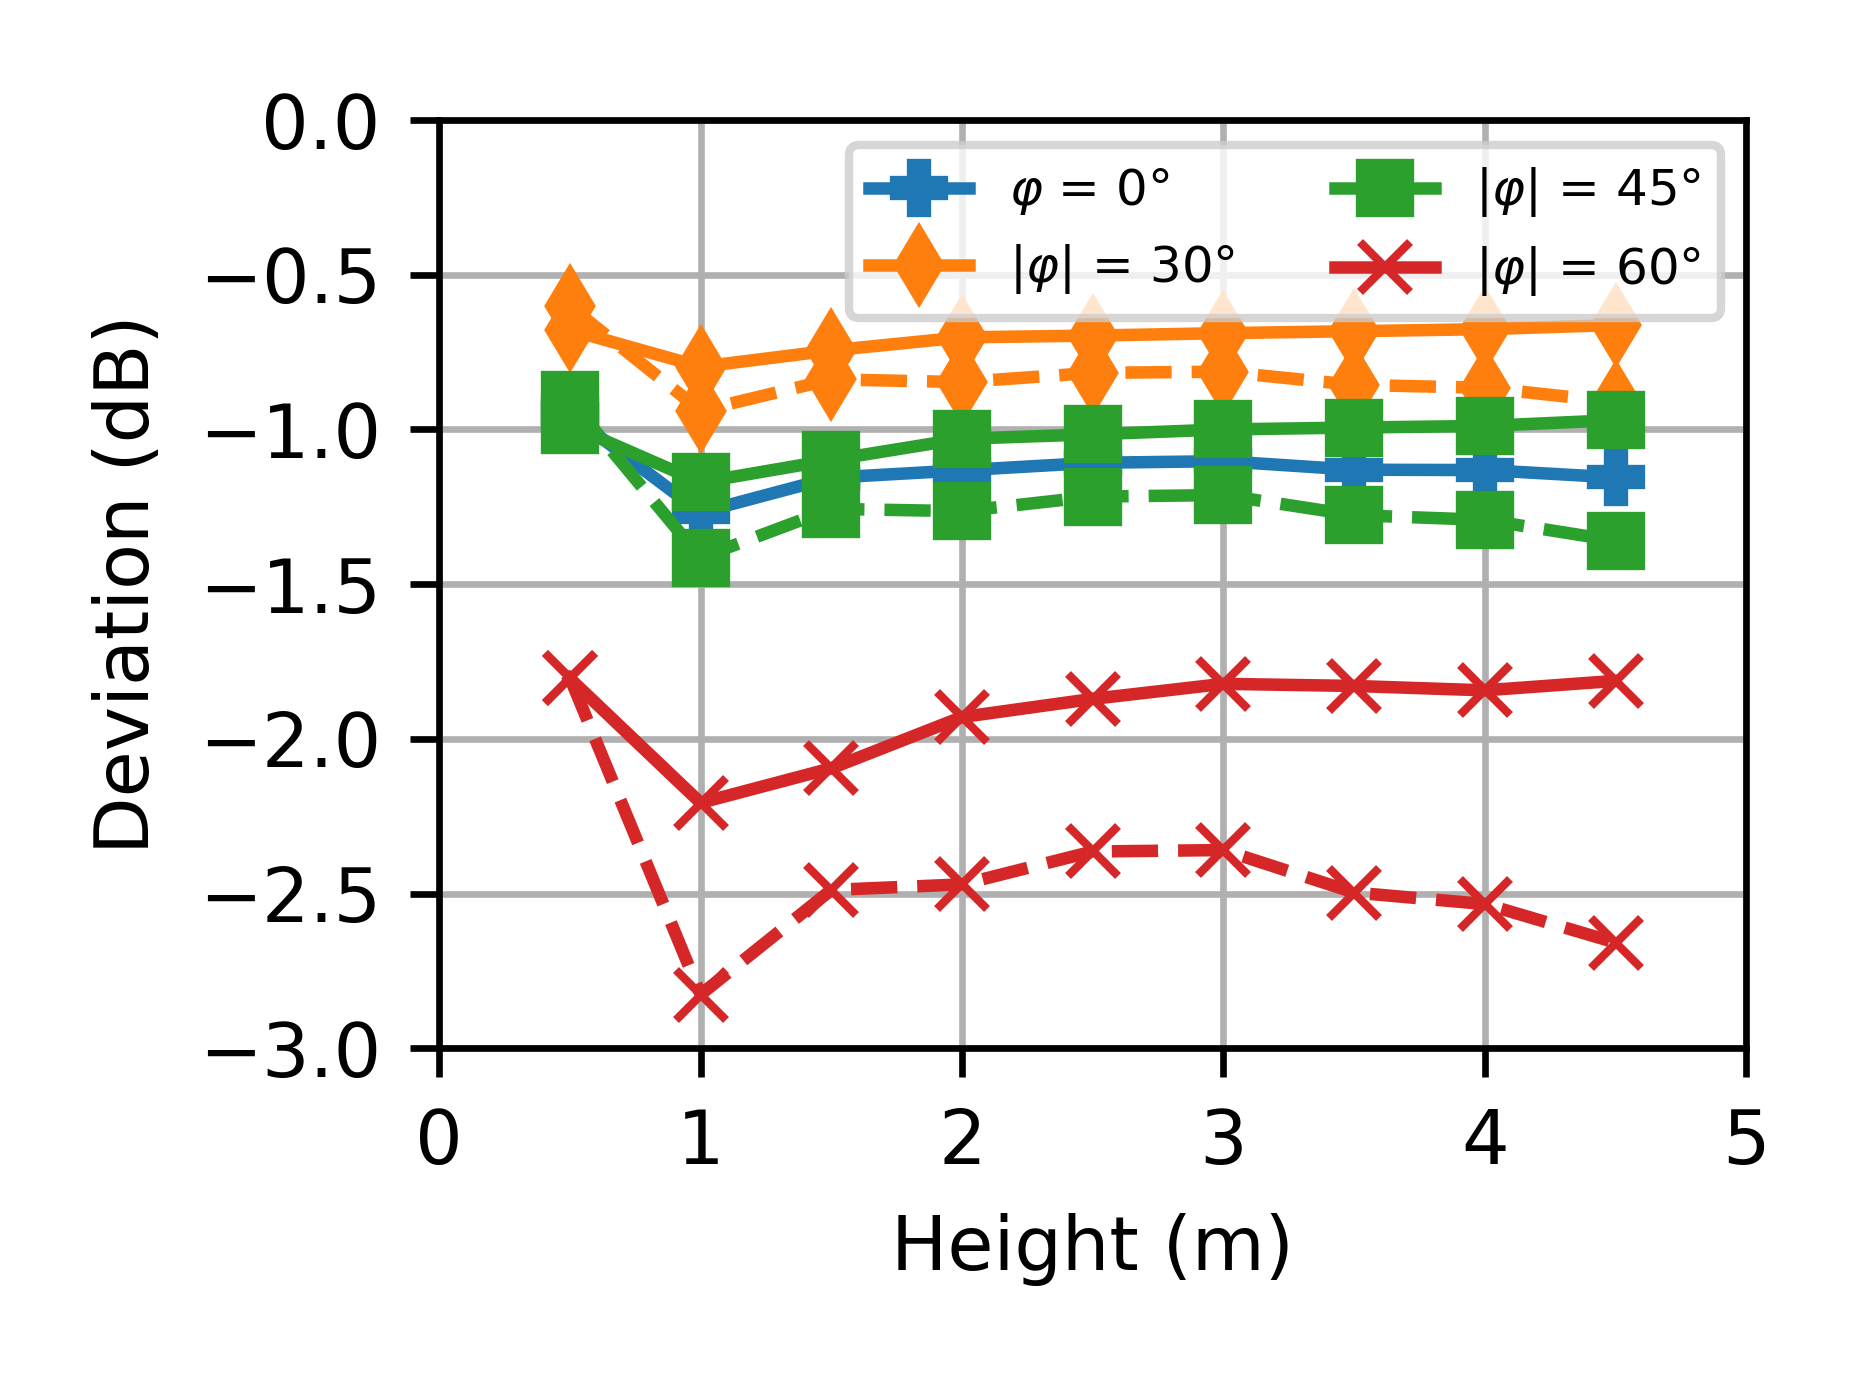
\includegraphics{fig/chap5/impedance/third_octave/deviation_1000_Hz.png}
		\caption{\SI{1000}{\hertz}}
	\end{subfigure}
	\\
	\begin{subfigure}[b]{\textwidth}
		\centering
		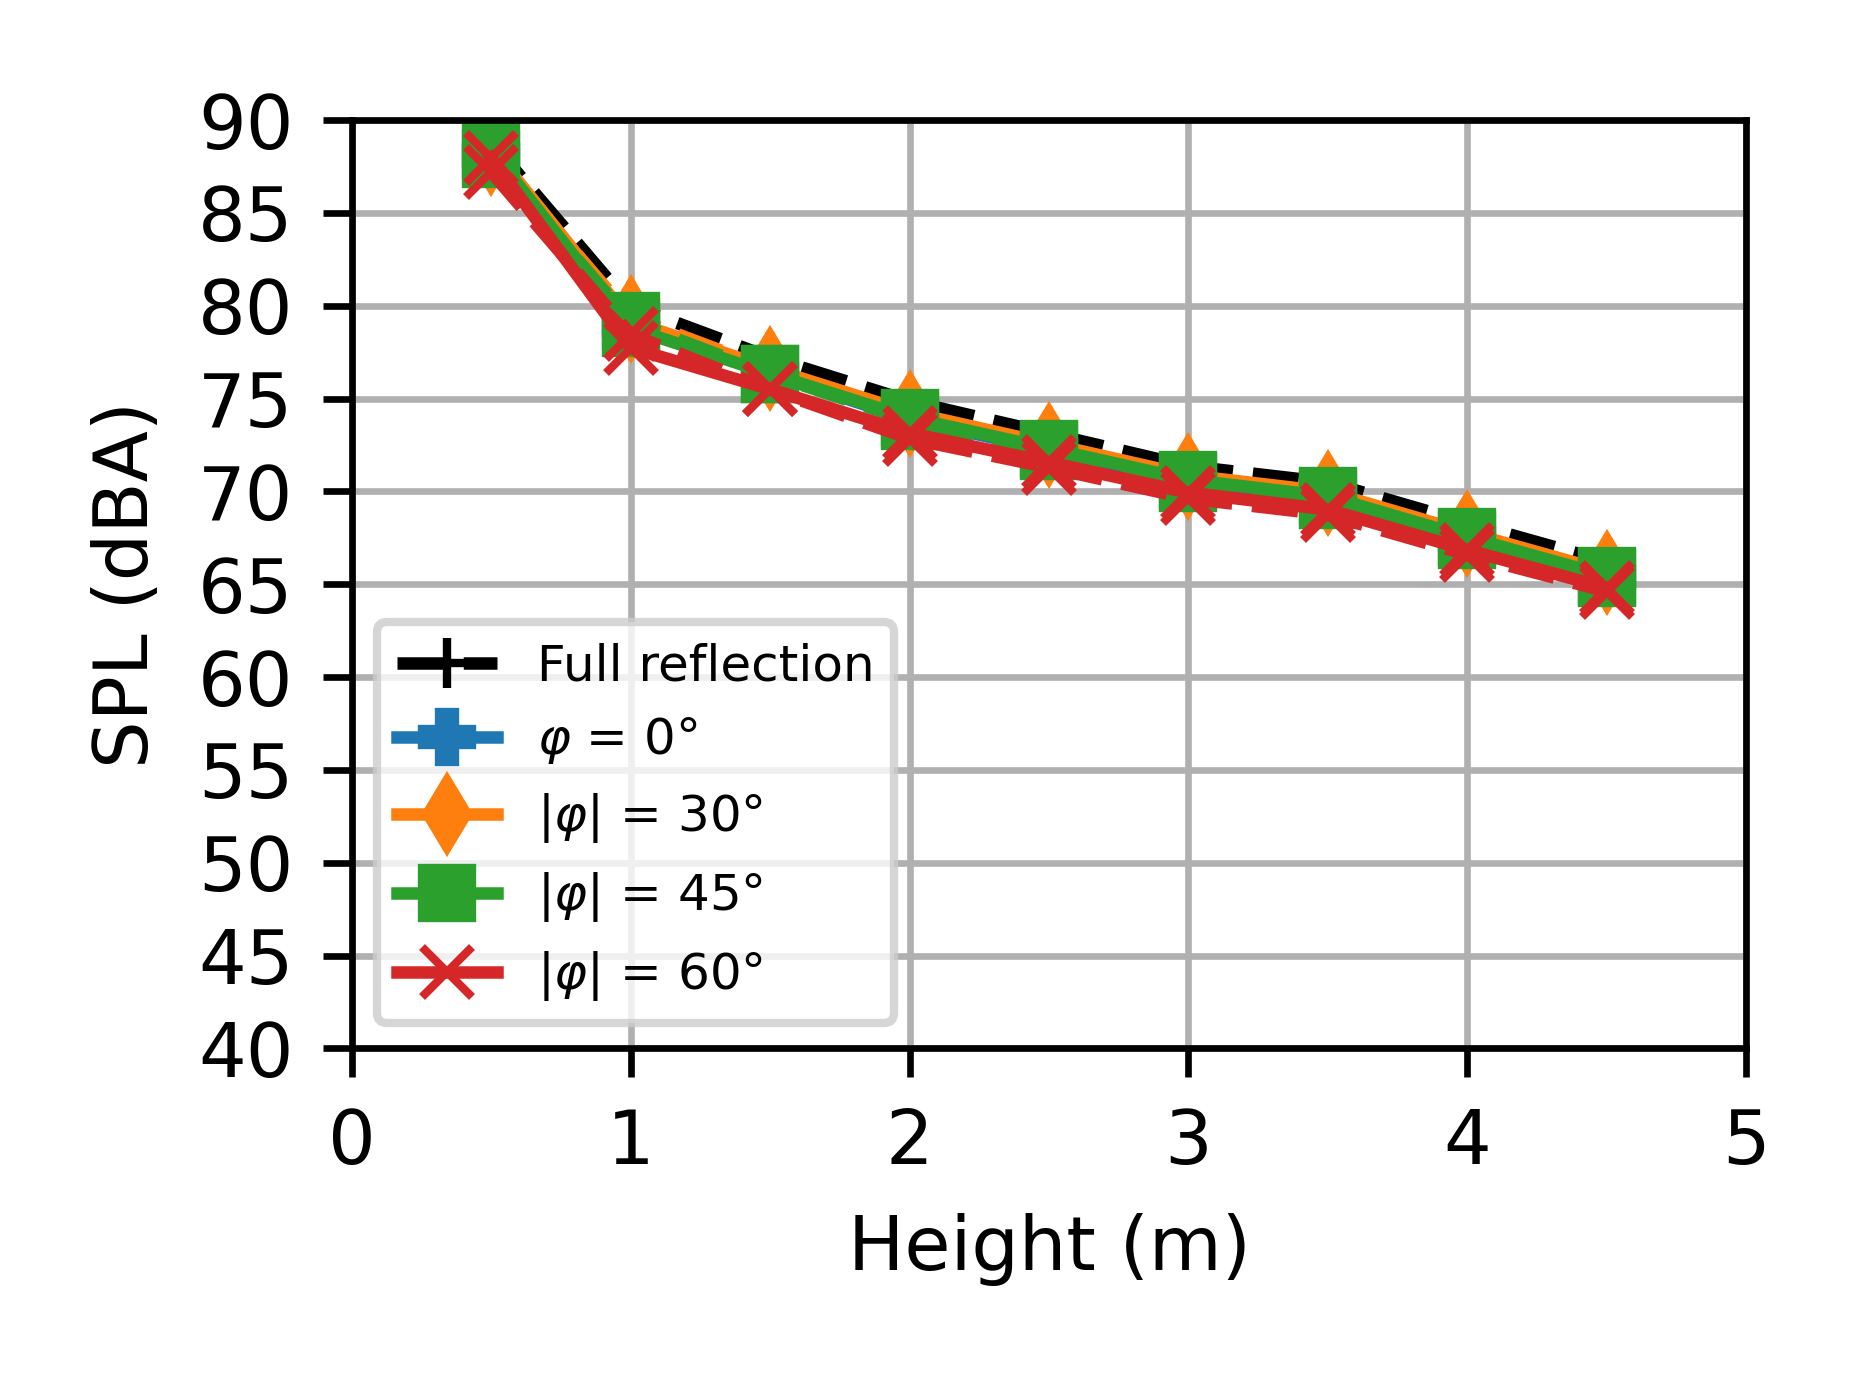
\includegraphics{fig/chap5/impedance/third_octave/SPL_2000_Hz.png}
		\hfill
		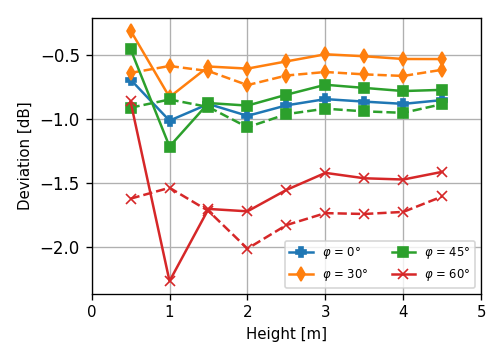
\includegraphics{fig/chap5/impedance/third_octave/deviation_2000_Hz.png}
		\caption{\SI{2000}{\hertz}}
	\end{subfigure}

	\caption{Sound distribution over the height at measurement position a, comparison between the model with full reflective ground (black dashed lines) and the models with different impedance phase angles (colored lines). Colored solid curves: positive phase angle; Colored dashed curves: negative phase angle.}
	\label{fig:third_octave_over_height_impedance}
\end{figure}

\Cref{fig:third_octave_over_height_impedance} shows the A-weighted sound pressure level at measurement position a (\SI{10}{\centi\meter} away from vehicle) along the carbody height for models with different impedance phase angles in example one third octave bands. The simulation results are compared to the result obtained by the model without ground absorption (initial model) and the difference is also shown in the figures.
As can be seen from the results, for \SI{100}{\hertz}, there is almost no noticeable difference between the absorption models and the initial model due to the small absorption coefficient (\SI{2}{\percent}) in the low frequency range from \SIrange{100}{250}{\hertz}. For frequencies with higher absorption coefficients, a decrease in sound pressure level due to absorption becomes more visible. One can see that the degree of absorption within a frequency band strongly depends on the phase angle of the complex surface impedance. In general, the greater the impedance angle the stronger the absorption. An exception exists for the model with zero phase angle, which contains only a real valued part, its curve lies between those of positive and negative 45-degree angles. Also, it can be seen that the attenuation also depends on the sign of the impedance phase angle, the negative angle (dashed line) leads to a slightly stronger attenuation than its complex conjugate (solid line), and the difference between the complex conjugate pair grows with the absolute phase angle. For phase angles with the same sign, they share the same curve shape, and only differ in their absolute values.

\begin{figure}
	\centering
	\begin{subfigure}[b]{\textwidth}
		\centering
		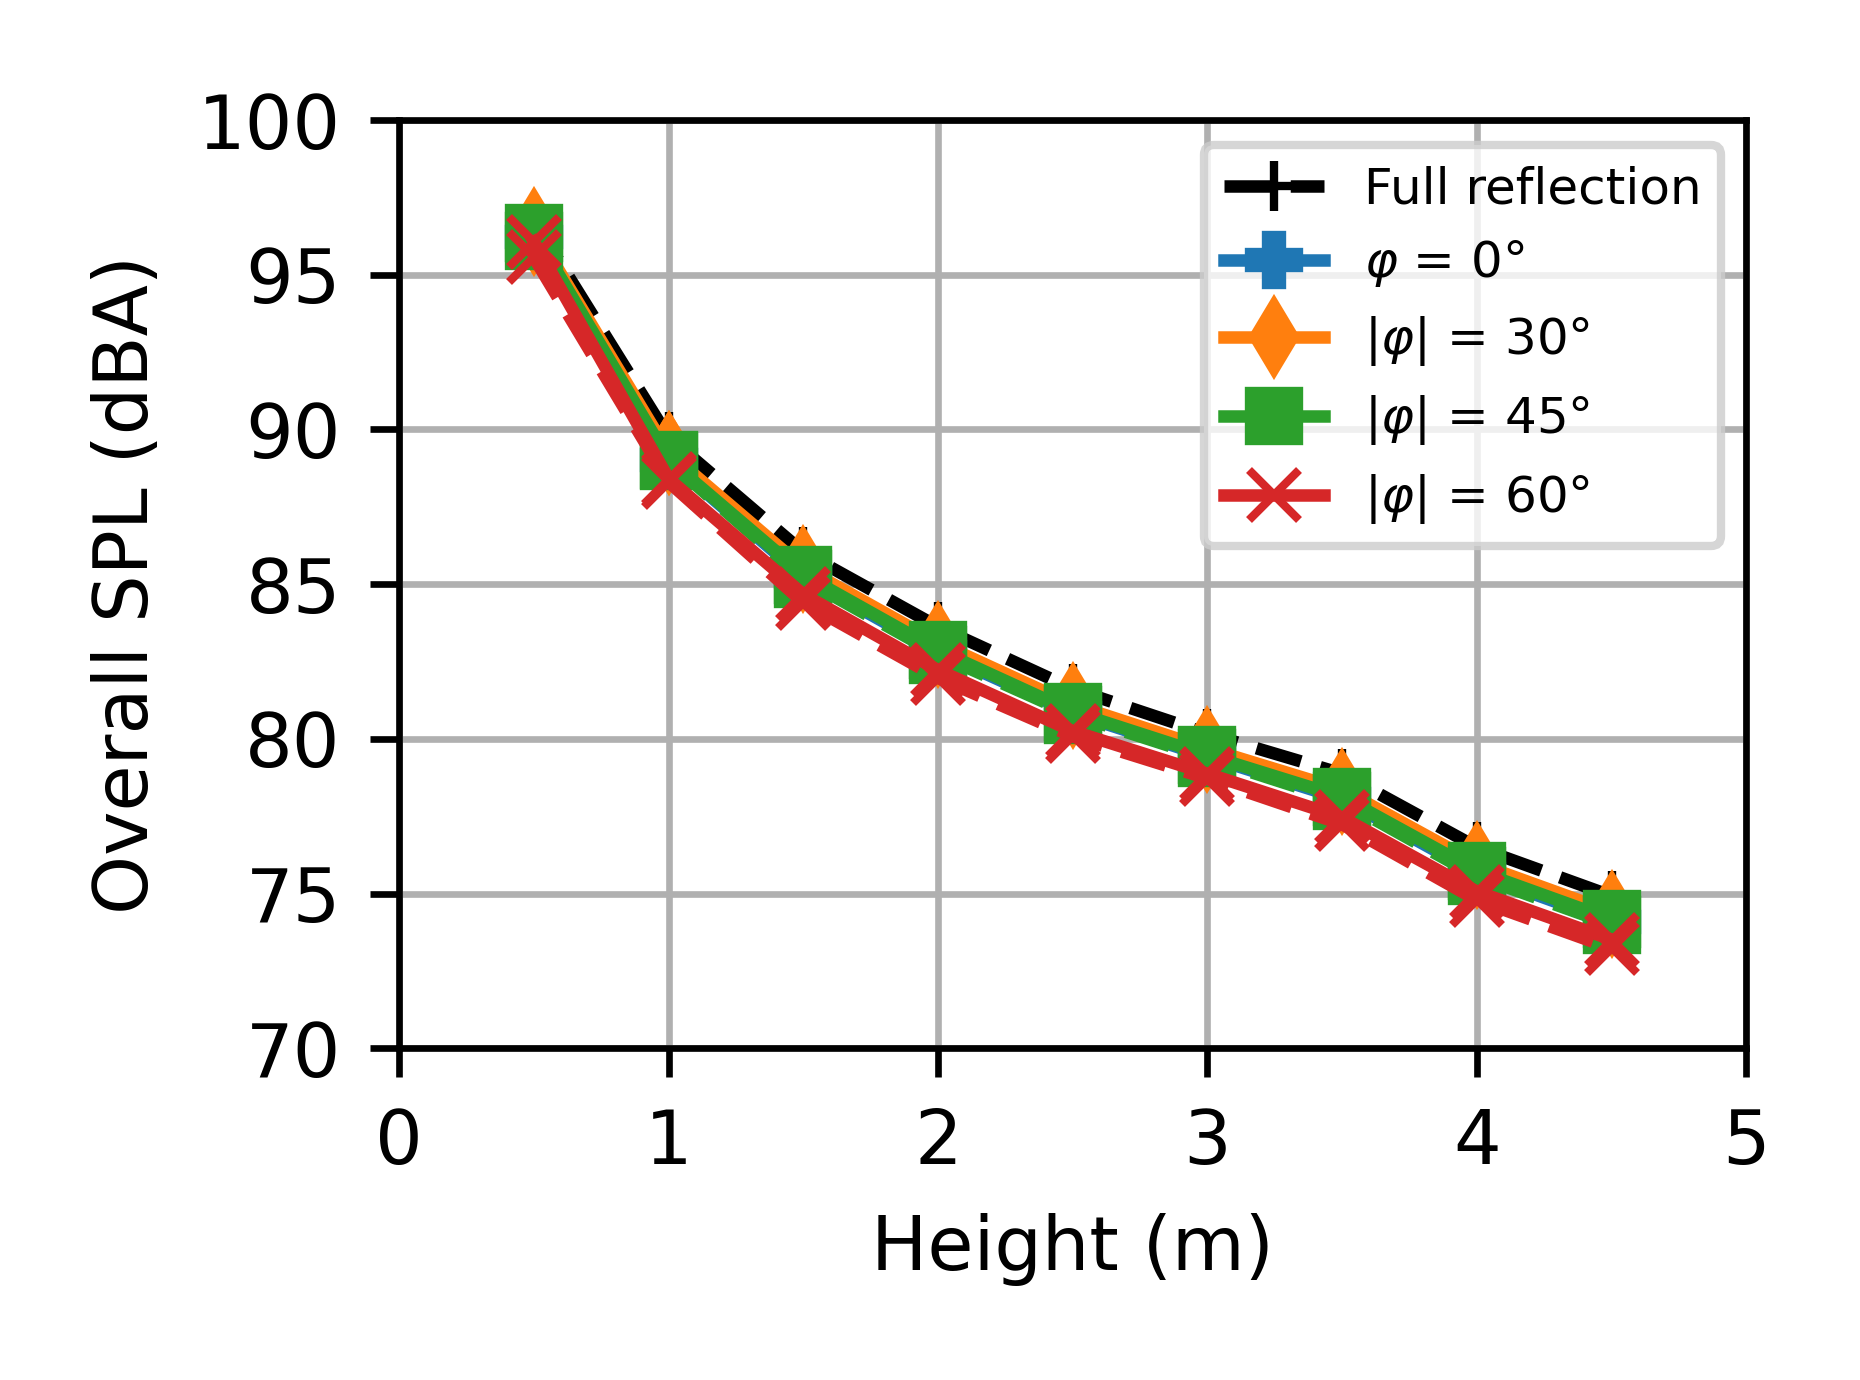
\includegraphics{fig/chap5/impedance/overall_SPL/overall_SPL_pos_a.png}
		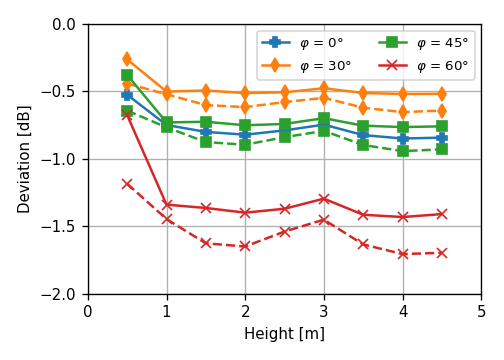
\includegraphics{fig/chap5/impedance/overall_SPL/deviation_pos_a.png}
		\caption{\SI{10}{\centi\meter} away from the car body}
	\end{subfigure}
	\\
	\begin{subfigure}[b]{\textwidth}
		\centering
		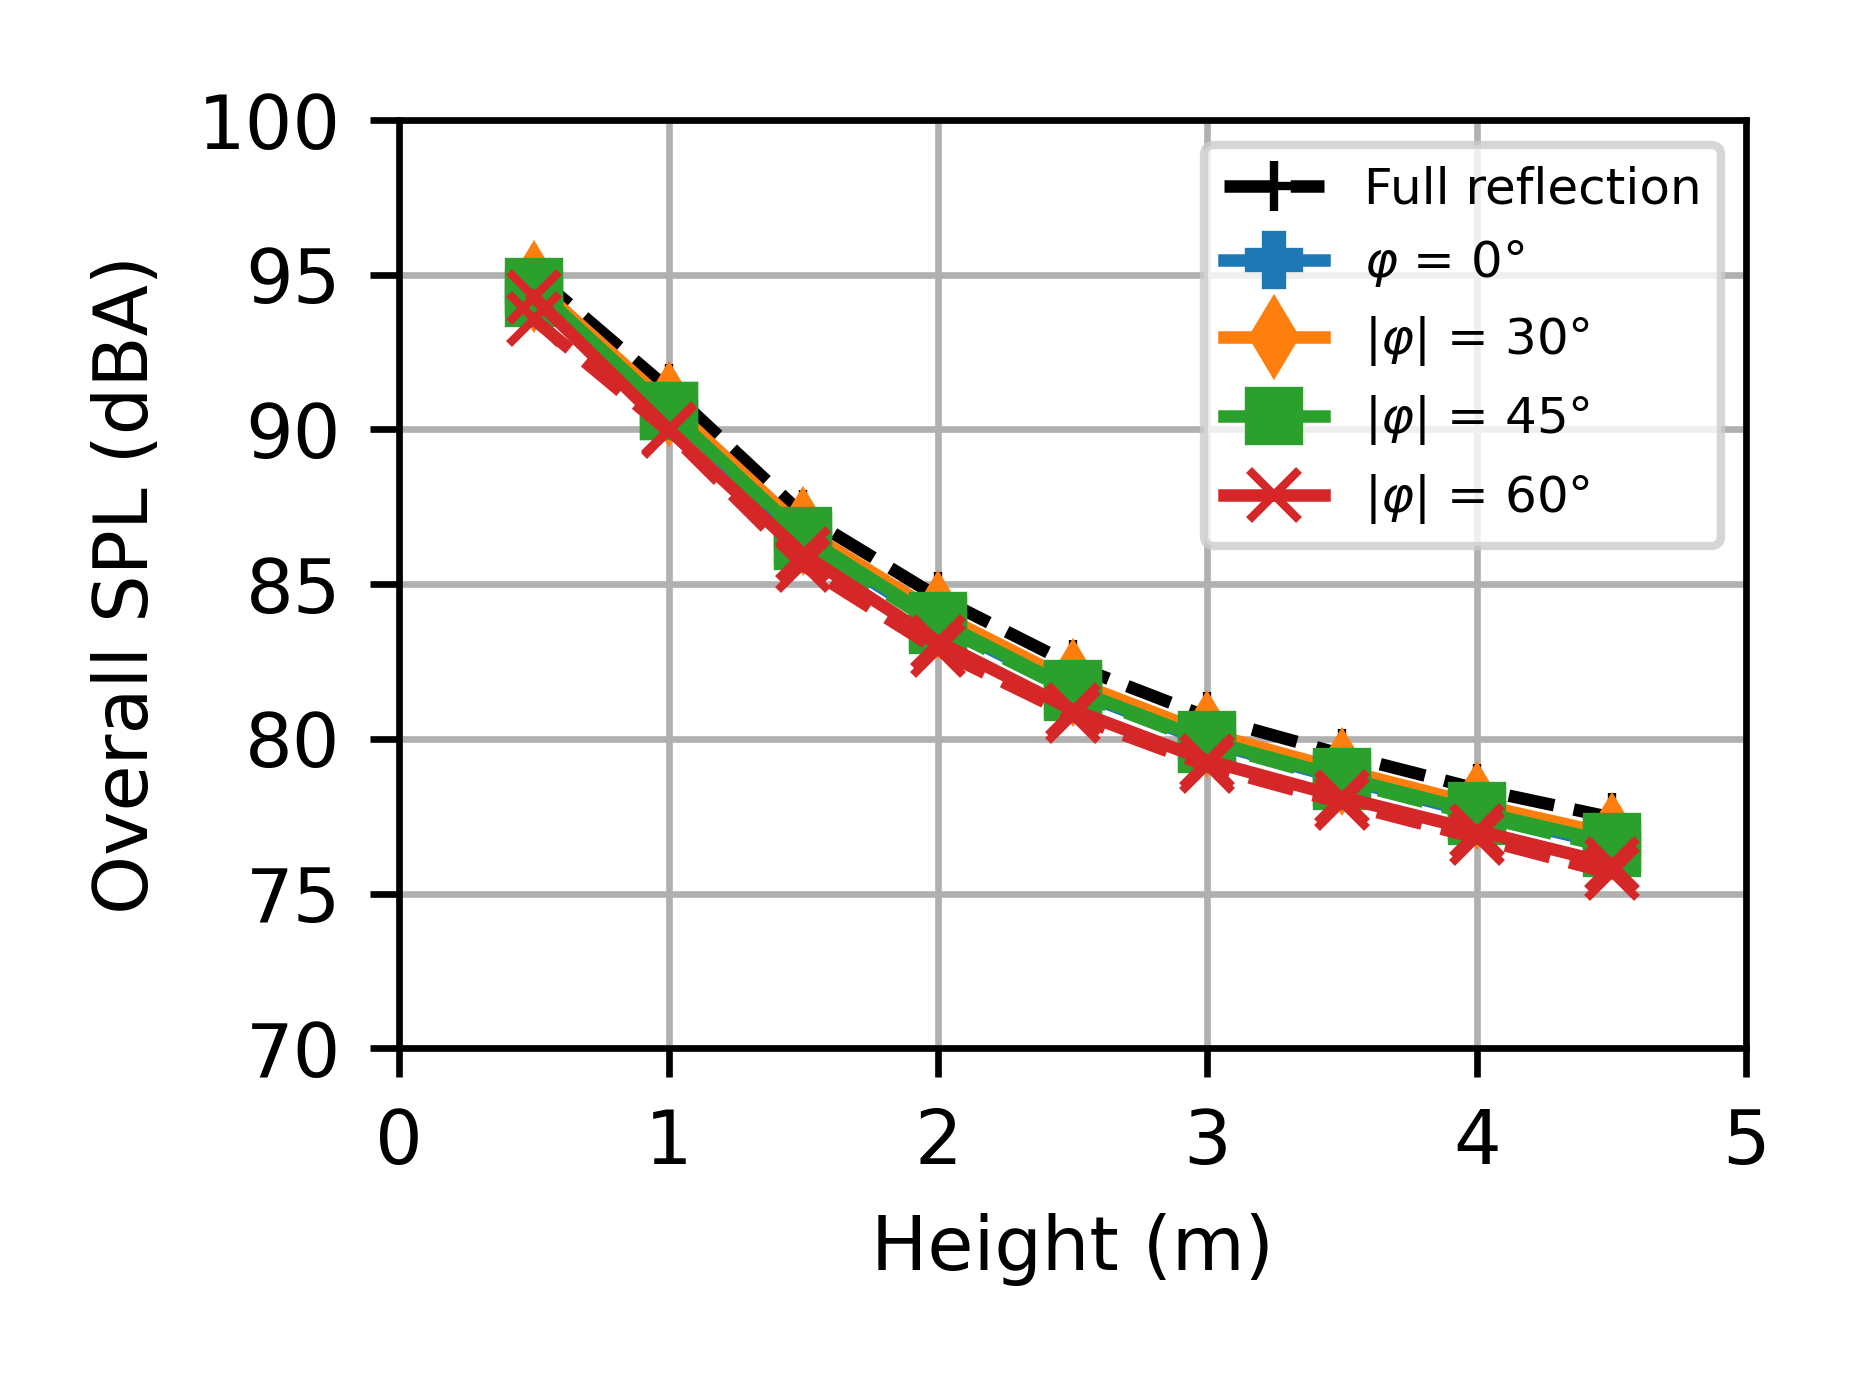
\includegraphics{fig/chap5/impedance/overall_SPL/overall_SPL_pos_f.png}
		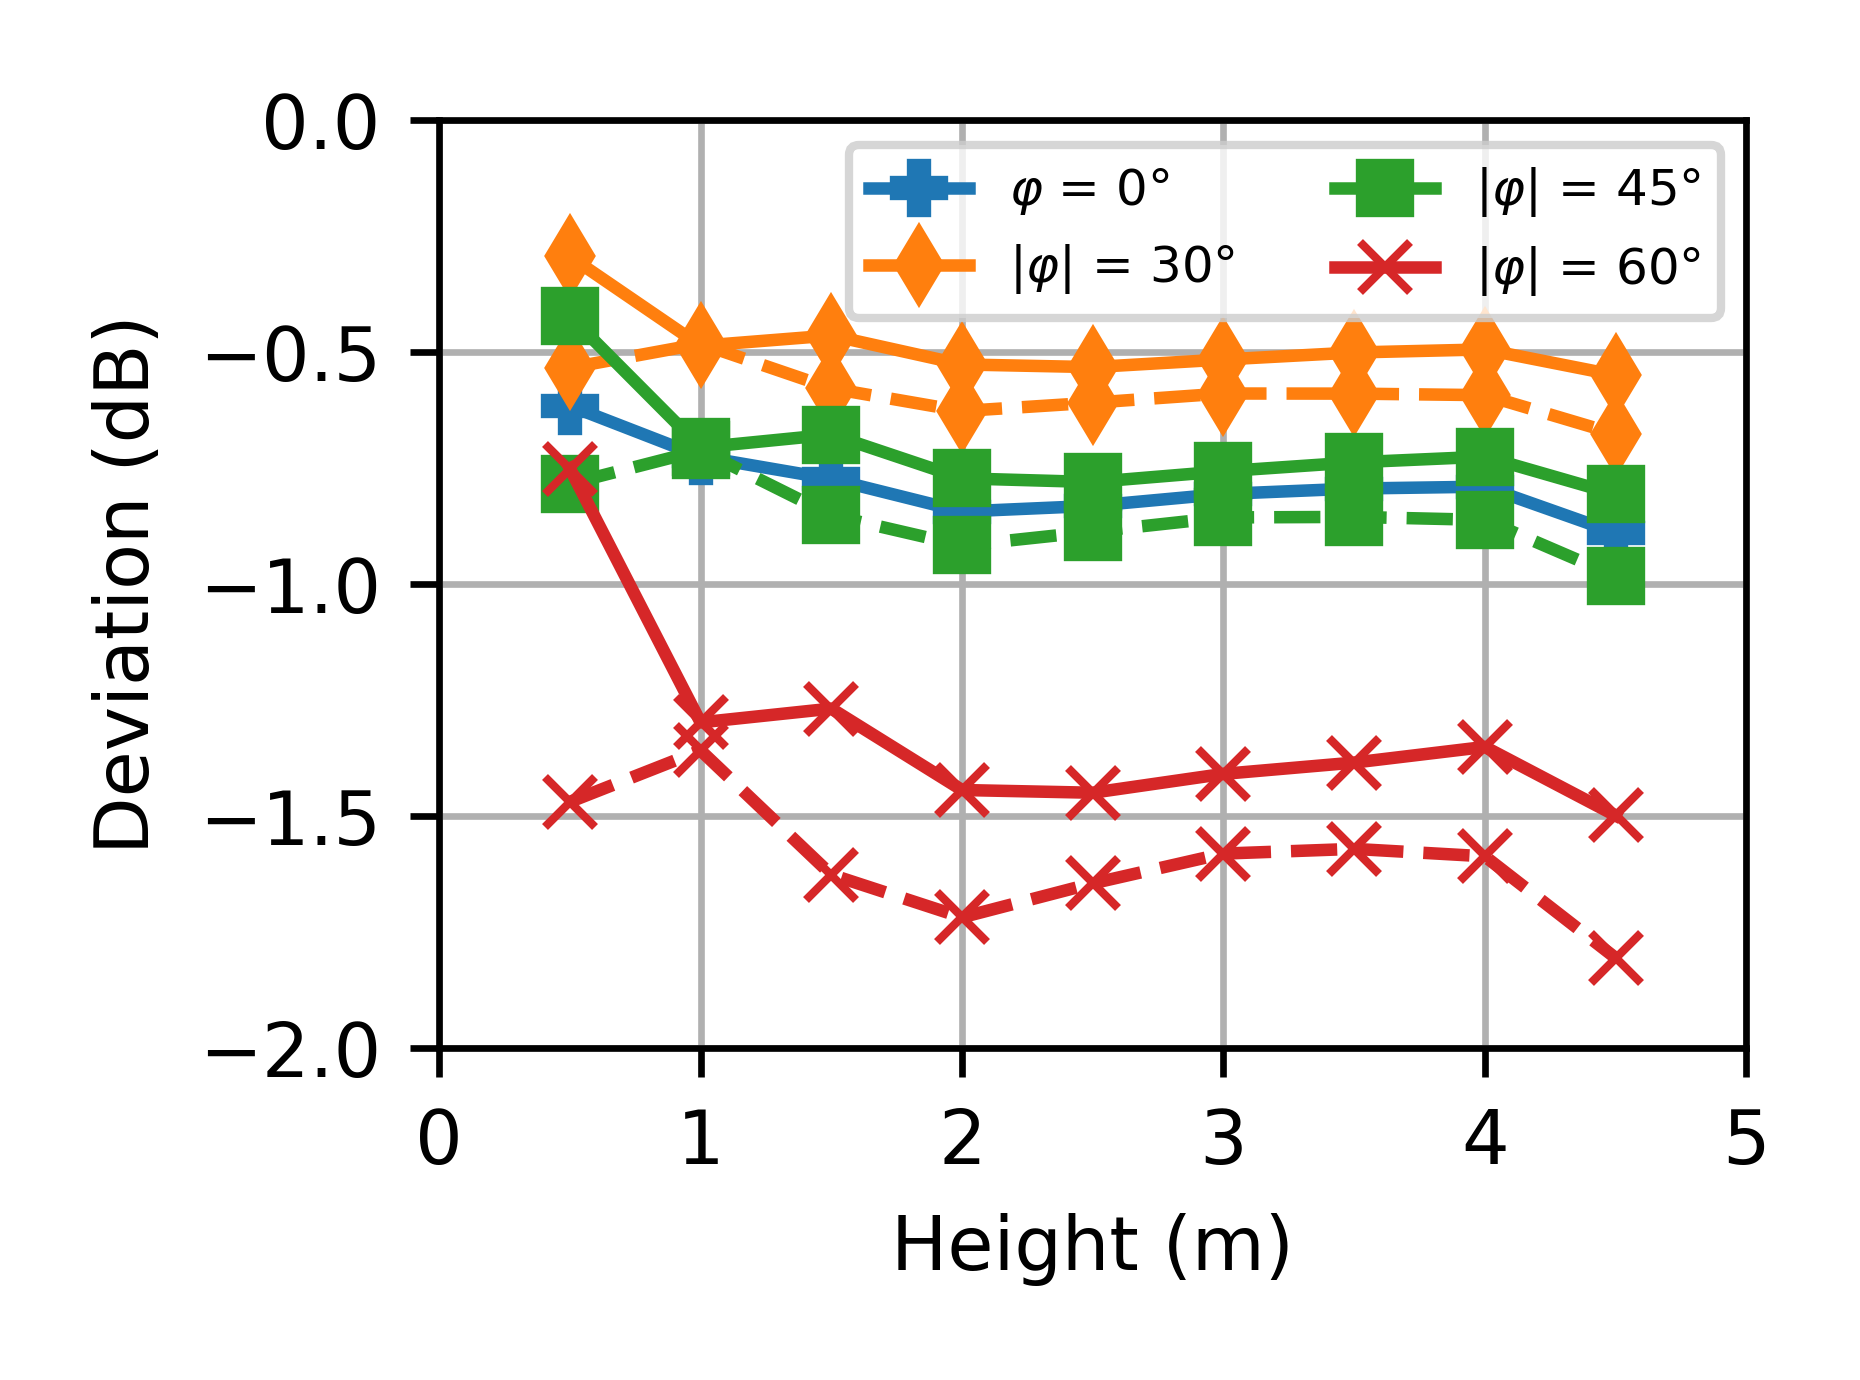
\includegraphics{fig/chap5/impedance/overall_SPL/deviation_pos_f.png}
		\caption{\SI{50}{\centi\meter} away from the carbody}
	\end{subfigure}
	\\
	\begin{subfigure}[b]{\textwidth}
		\centering
		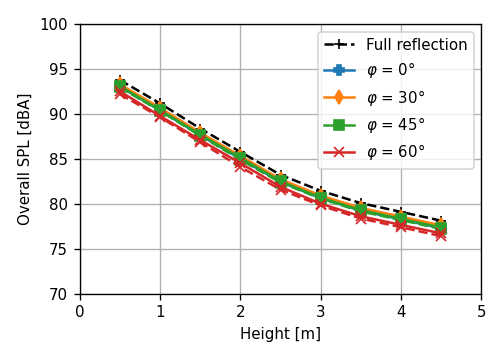
\includegraphics{fig/chap5/impedance/overall_SPL/overall_SPL_pos_g.png}
		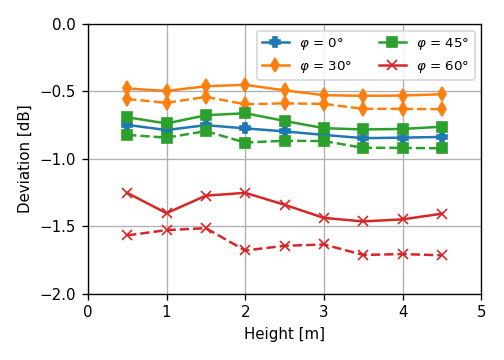
\includegraphics{fig/chap5/impedance/overall_SPL/deviation_pos_g.png}
		\caption{\SI{100}{\centi\meter} away from the carbody}
	\end{subfigure}
	
	\caption{Comparison of overall A-weighted sound pressure level between difference impedance phase angles at various measurement positions. Solid lines: positive phase angle; dashed lines: negative phase angle.}
	\label{fig:overall_SPL_impedance}
\end{figure}

Very similar results are also observed in the overall sound pressure level distribution, which is shown in \cref{fig:overall_SPL_impedance}. Again, the impedance phase angle dependency of the absorption can be seen from the results, i.e., the greater the phase angle, the greater the deviation to the full reflective model and hence, the higher the attenuation. The greatest difference in terms of overall sound pressure level among the investigated phase angles is about \SI{1}{\decibel}. Furthermore, a complex conjugate pair with the same absolute impedance phase angle with a negative phase angle (dashed line) shows higher attenuation than the positive one (solid line). Furthermore, the deviation among the conjugate pair grows with the absolute phase angle. In the case of zero phase angle whose surface impedance contains only real part, its result lies between those of the 45-degree complex conjugate pair.

\begin{figure}
	\centering
	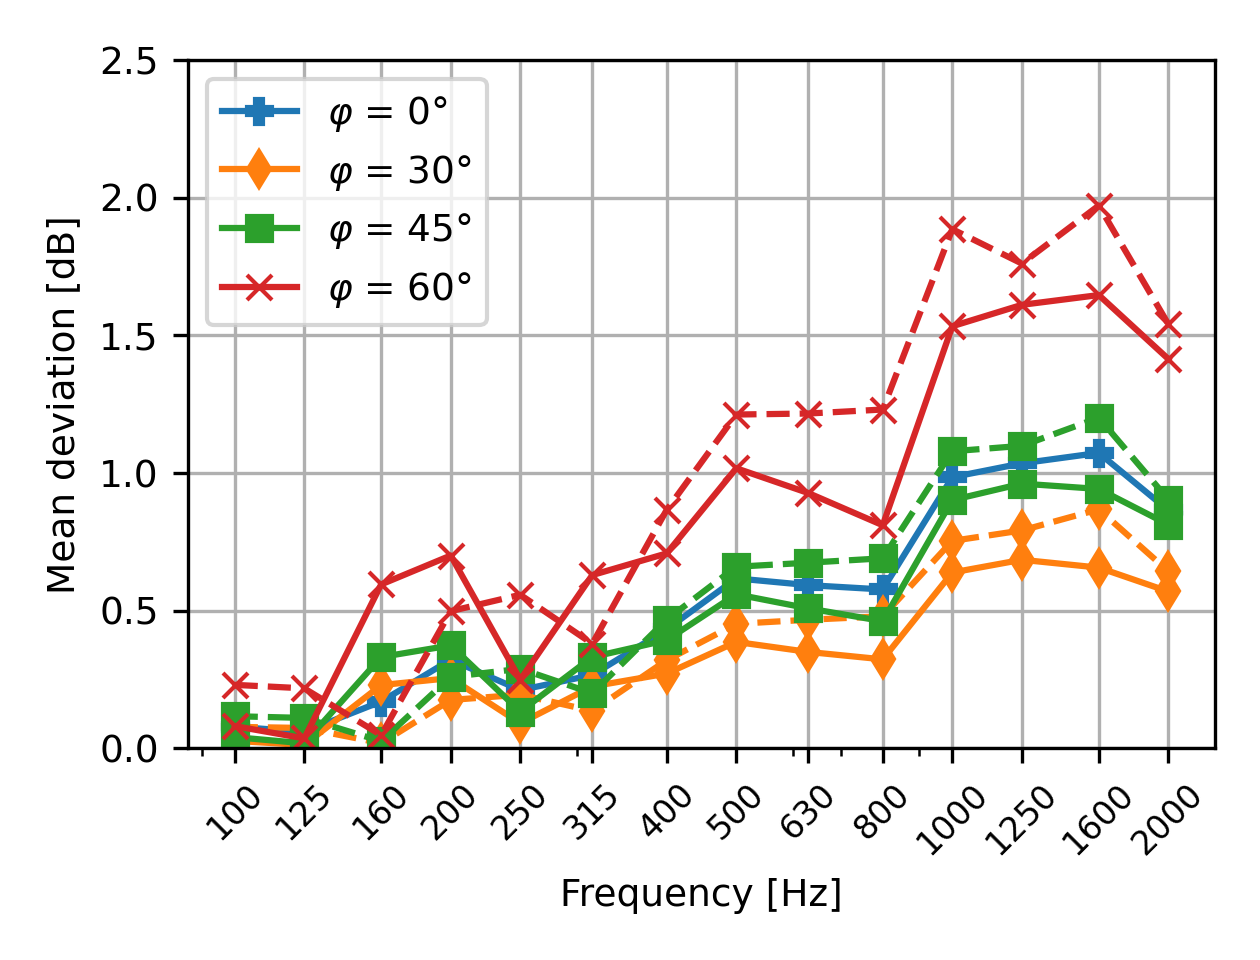
\includegraphics[width=0.7\linewidth]{fig/chap5/impedance/freq_spectrum/average_gap.png}
	\caption{Mean relative deviation in terms of sound pressure level compared to full reflective model in 1/3-octave bands. Solid lines: positive phase angle; dashed lines: negative phase angle.}
	\label{fig:gap_freq_spectrum_impedance}
\end{figure}

\Cref{fig:gap_freq_spectrum_impedance} shows the mean relative deviation spectra in terms of sound pressure level for different impedance phase angles compared to the initial model with fully reflective ground. As can be seen from the results, in low frequency region between \SI{100}{\hertz} and \SI{315}{\hertz}, where the absorption coefficient is small (\SIrange{2}{3}{\percent}), the difference in results between the different phase angles is also small. With growing absorption coefficient, the deviation between the phase angles gets larger. The largest difference occurs in the high frequency region, in this case between \SI{1000}{\hertz} and \SI{2000}{\hertz}, where the deviation is about \SI{1.5}{\decibel}.

\begin{table}
	\centering
	\caption{Mean deviation in overall SPL for different impedance phase angles.}
	\label{tab:mean_devaition_impedance}
	\begin{tabular}{cc}
		\toprule
		$\text{arg}(\tilde{R_s} + j\tilde{X_s})$ (°) & Average deviation in overall SPL (dB) \\
		\midrule
		0                         & 0.72                                      \\
		30/-30                    & 0.46/0.55                                 \\
		45/-45                    & 0.66/0.78                                 \\
		60/-60                    & 1.15/1.34                                 \\
		\bottomrule
	\end{tabular}
\end{table}

The average deviation in terms of overall sound pressure level compared to the full reflective model can be found in \cref{tab:mean_devaition_impedance}. A larger deviation to full reflective model means a larger absorption of the sound pressure. One can see that the difference between the smallest and the largest absorption degree is about \SI{1}{\decibel}. Additionally, the absorptance of 0-degree angle is the median of the result set.

From the results shown in this section it can be concluded that for a given normal incident absorption coefficient spectrum, the actual attenuation of the acoustic wave depends on the phase angle of the complex surface impedance. For a given absorption coefficient with a value of 0.1, the actual attenuation of the pressure obtained varies from about \SI{0.5}{\decibel} to \SI{2}{\decibel} depending on the investigated impedance phase angles. In cases where only data for the absorption coefficient is available, it can be assumed that the surface impedance contains only a real part. The same approach is also used by Li et al. \cite{li_25d_2021} in their finite element analysis for rail acoustics to handle the unknown impedance phase angle. In order to obtain a more accurate simulation result, not only should the absorption spectrum of the material be provided, but also the full impedance characteristic of the ground surface. This information can be obtained by, e.g., an in-situ measurement of surface impedance using impedance tube method as described in \cite{hald_situ_2019, wolkesson_2013}.

\section{Effect of varying frequency steps per 1/3-octave band}

In this section, the simulation results obtained by variation analysis using different intermediate frequency steps in single 1/3-octave band are shown.

\begin{figure}
	\centering
	\begin{subfigure}[b]{0.49\textwidth}
		\centering
		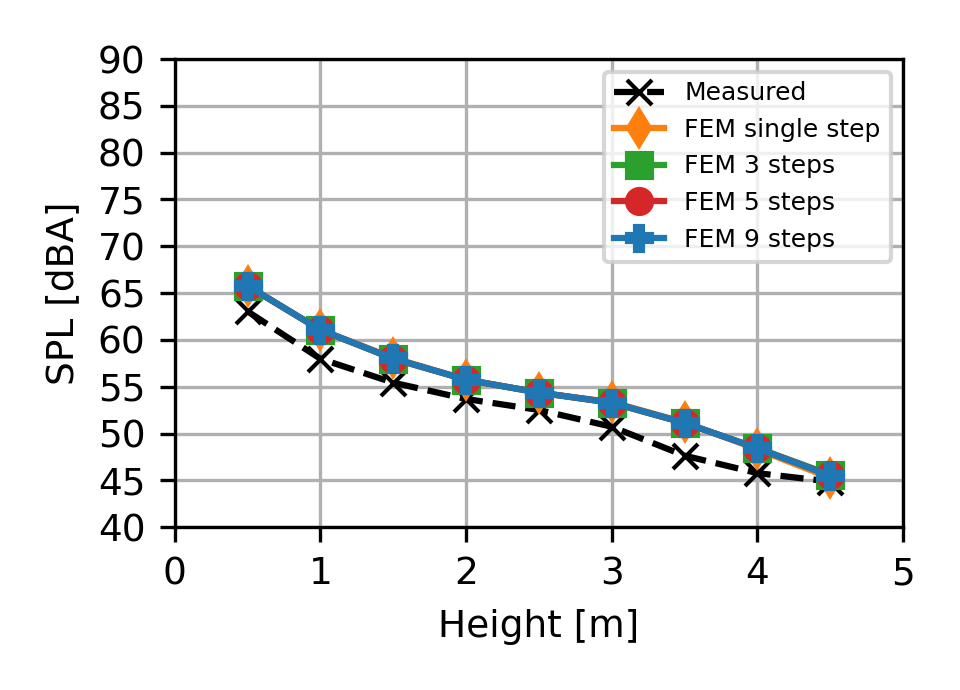
\includegraphics{fig/chap5/freq_steps/third_octave_over_height/100_Hz.png}
		\caption{\SI{100}{\hertz}}
	\end{subfigure}
	\hfill
	\begin{subfigure}[b]{0.49\textwidth}
		\centering
		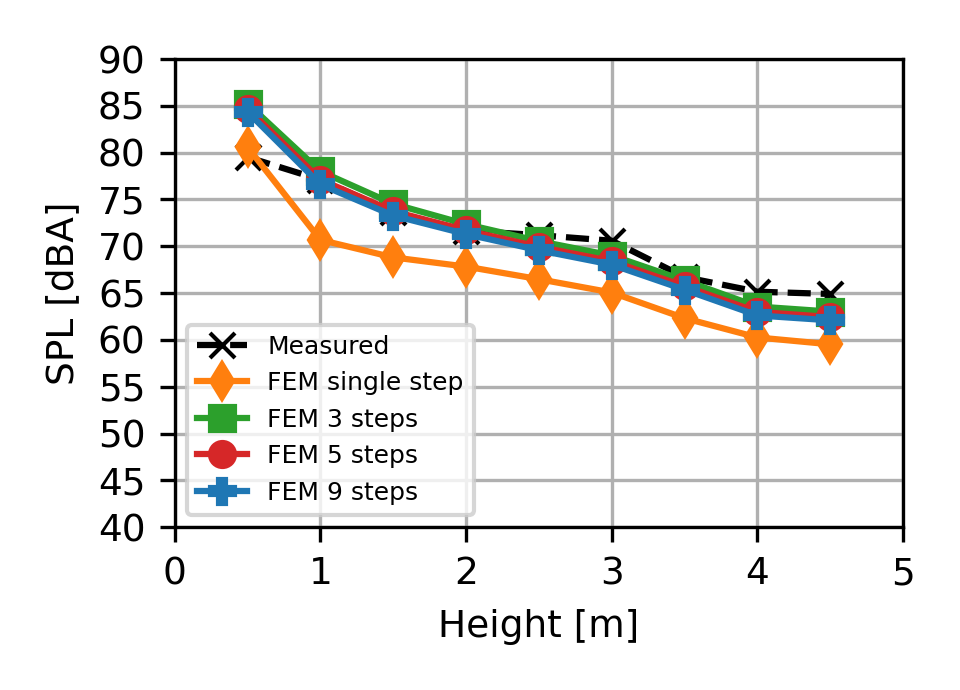
\includegraphics{fig/chap5/freq_steps/third_octave_over_height/315_Hz.png}
		\caption{\SI{315}{\hertz}}
	\end{subfigure}
	\\
	\begin{subfigure}[b]{0.49\textwidth}
		\centering
		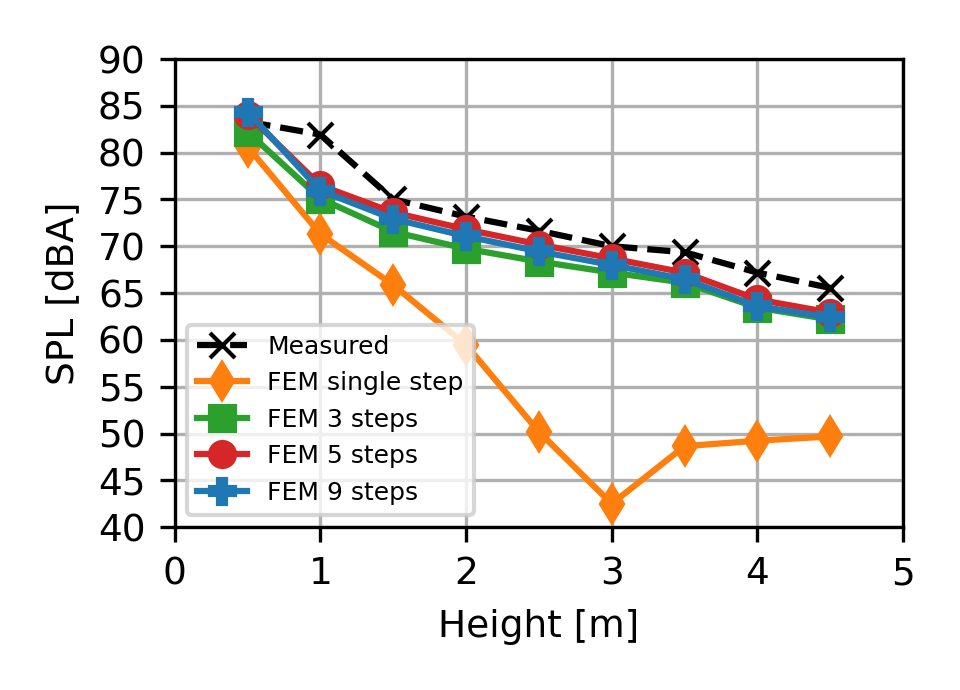
\includegraphics{fig/chap5/freq_steps/third_octave_over_height/630_Hz.png}
		\caption{\SI{630}{\hertz}}
	\end{subfigure}
	\hfill
	\begin{subfigure}[b]{0.49\textwidth}
		\centering
		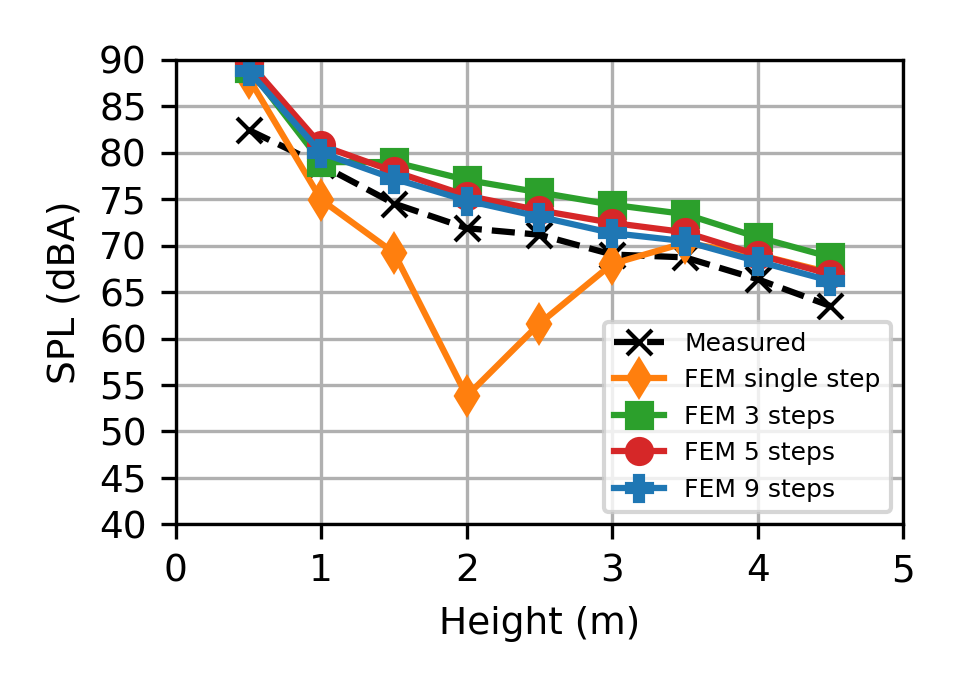
\includegraphics{fig/chap5/freq_steps/third_octave_over_height/2000_Hz.png}
		\caption{\SI{2000}{\hertz}}
		\label{fig:curve_sink}
	\end{subfigure}
	
	\caption{A-weighted sound pressure level over the height at measurement position a, comparison between measurement (dash lines) and simulation (solid lines) using different intermediate steps per one-third octave band.}
	
	\label{fig:third_octave_over_height_freq_steps}
\end{figure}

\Cref{fig:third_octave_over_height_freq_steps} shows the sound distribution at measurement position a (\SI{10}{\centi\meter} away from vehicle) along the height direction for different frequency resolutions of one-third octave bands. As can be seen from the results, there is almost no noticeable difference in results for \SI{100}{\hertz} between the different frequency steps due to its narrow bandwidth of about \SI{23}{\hertz}, and a high ratio of wavelength to geometry feature length could also be a reason. With increasing one-third octave band frequency and hence an increasing bandwidth, using one single intermediate frequency step to resolve the one-third octave band is not enough. At \SI{315}{\hertz}, the predicted sound pressure level using only a single step is about \SI{5}{\decibel} lower than the results obtained with more frequency steps. In the \SI{630}{\hertz} and \SI{2000}{\hertz} bands, when using only the center frequency to represent the one-third octave band, a destructive interference effect in the sound distribution can be observed. The sink in the sound pressure curve is smoothed out once more intermediate frequency steps are used to compute the one-third octave band result. Except for the single step, results obtained by using 3, 5 and 9 intermediate steps are in the same range and agree well with the measurement.

\begin{figure}
	\centering
	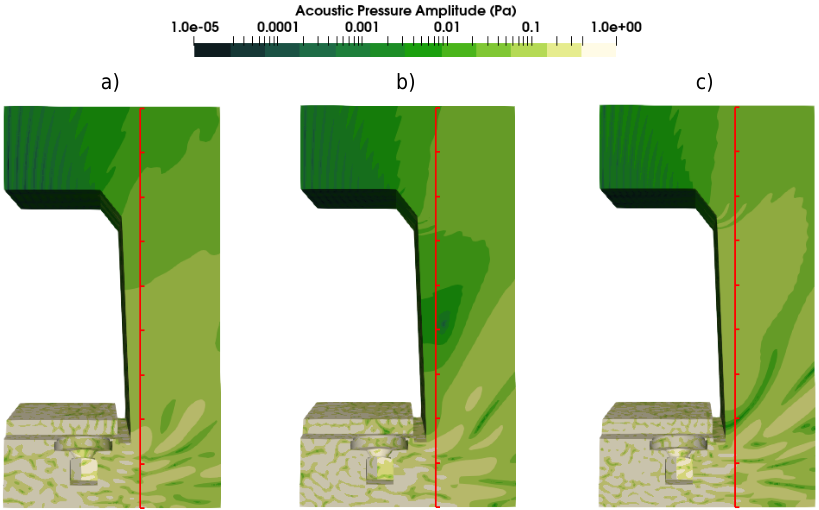
\includegraphics[width=\textwidth]{fig/chap5/freq_steps/field_result.png}
	\caption{Acoustic pressure amplitude field for three frequencies in \SI{2000}{\hertz} one-third octave band. a) \SI{1781}{\hertz}; b) \SI{2000}{\hertz}; c) \SI{2245}{\hertz}. The vertical red line indicates the evaluation position (\SI{10}{\centi\meter} from the car body) over the domain height.}
	\label{fig:pressure_field_solution}
\end{figure}

\Cref{fig:pressure_field_solution} shows the pressure field of three frequencies within the 2000 Hz one-third octave band. The frequencies are corresponding to the lower band limit, the center frequency and the upper band limit of the one-third octave band, respectively. The sink in the sound pressure level curve using only single step as shown in \cref{fig:curve_sink} is due to the destructive interference of the acoustic wave, which can be seen in the pressure field corresponding to \SI{2000}{\hertz}. The dark green at the middle of the carbody wall indicates a sink in the acoustic pressure. If more intermediate frequency steps are used, the sink in the sound pressure level curve will get averaged out since no destructive interference occurs at the same location in the pressure field of other frequencies.

\begin{figure}
	\begin{subfigure}[b]{\textwidth}
		\centering
		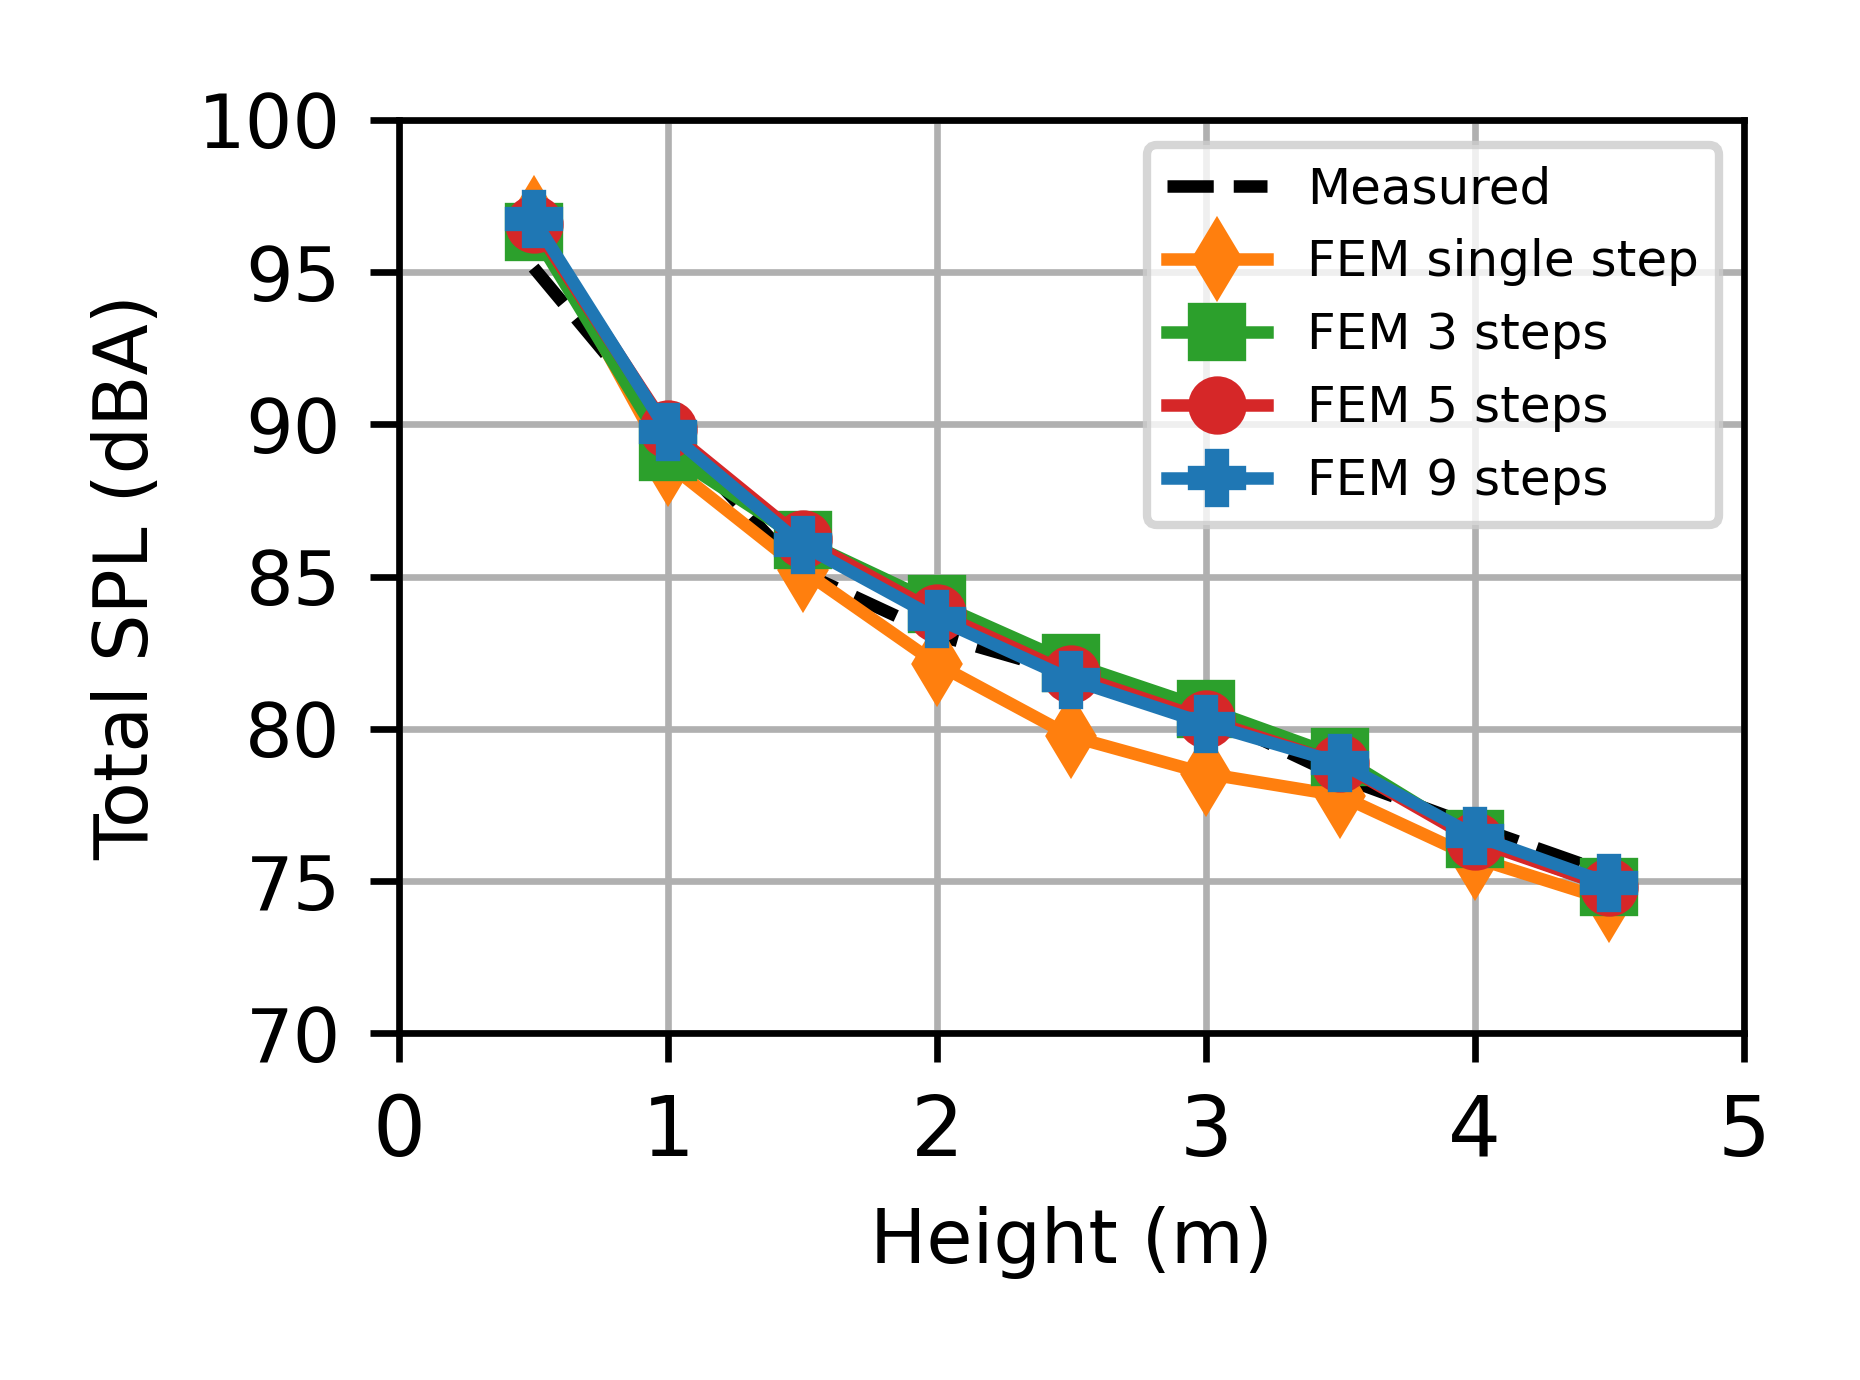
\includegraphics[width=0.49\textwidth]{fig/chap5/freq_steps/overall_SPL/pos_a.png}
		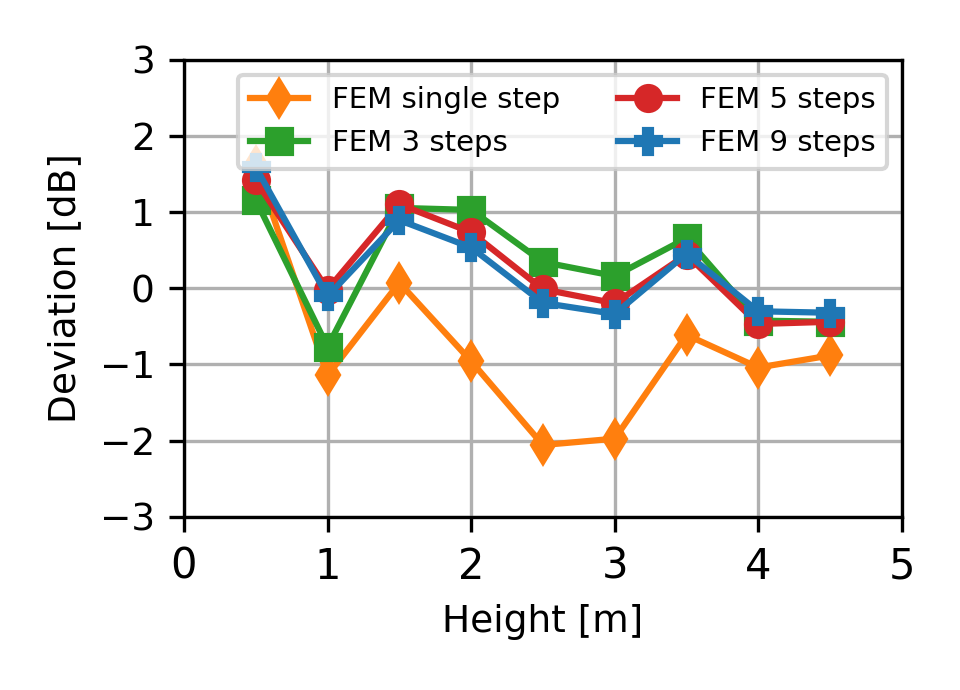
\includegraphics[width=0.49\textwidth]{fig/chap5/freq_steps/overall_SPL/pos_a_deviation.png}
		\caption{\SI{10}{\centi\meter} away from the carbody}
	\end{subfigure}

	\begin{subfigure}[b]{\textwidth}
		\centering
		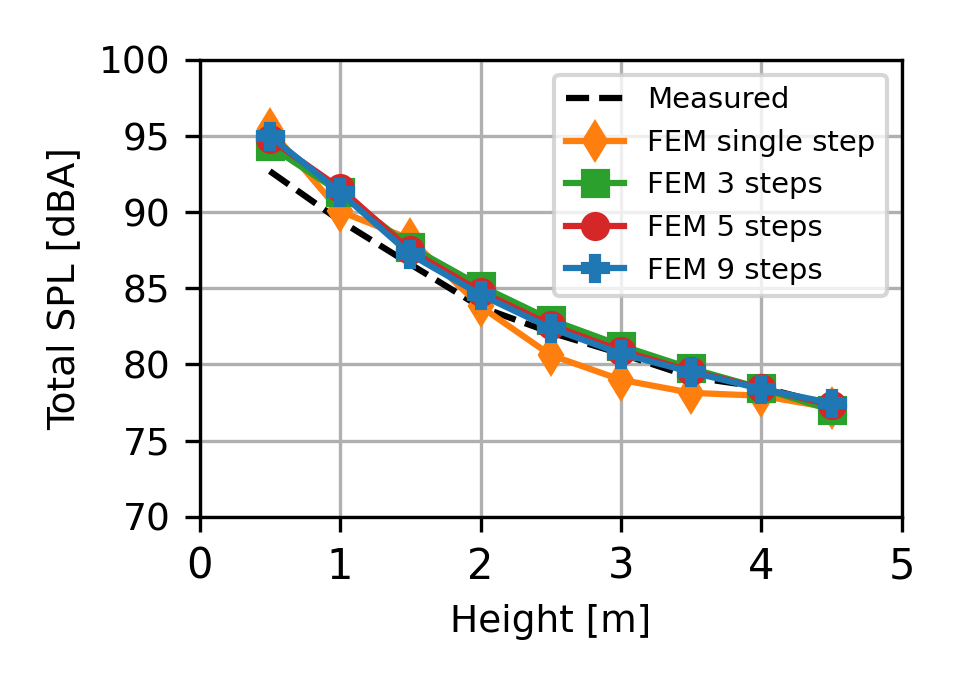
\includegraphics[width=0.49\textwidth]{fig/chap5/freq_steps/overall_SPL/pos_f.png}
		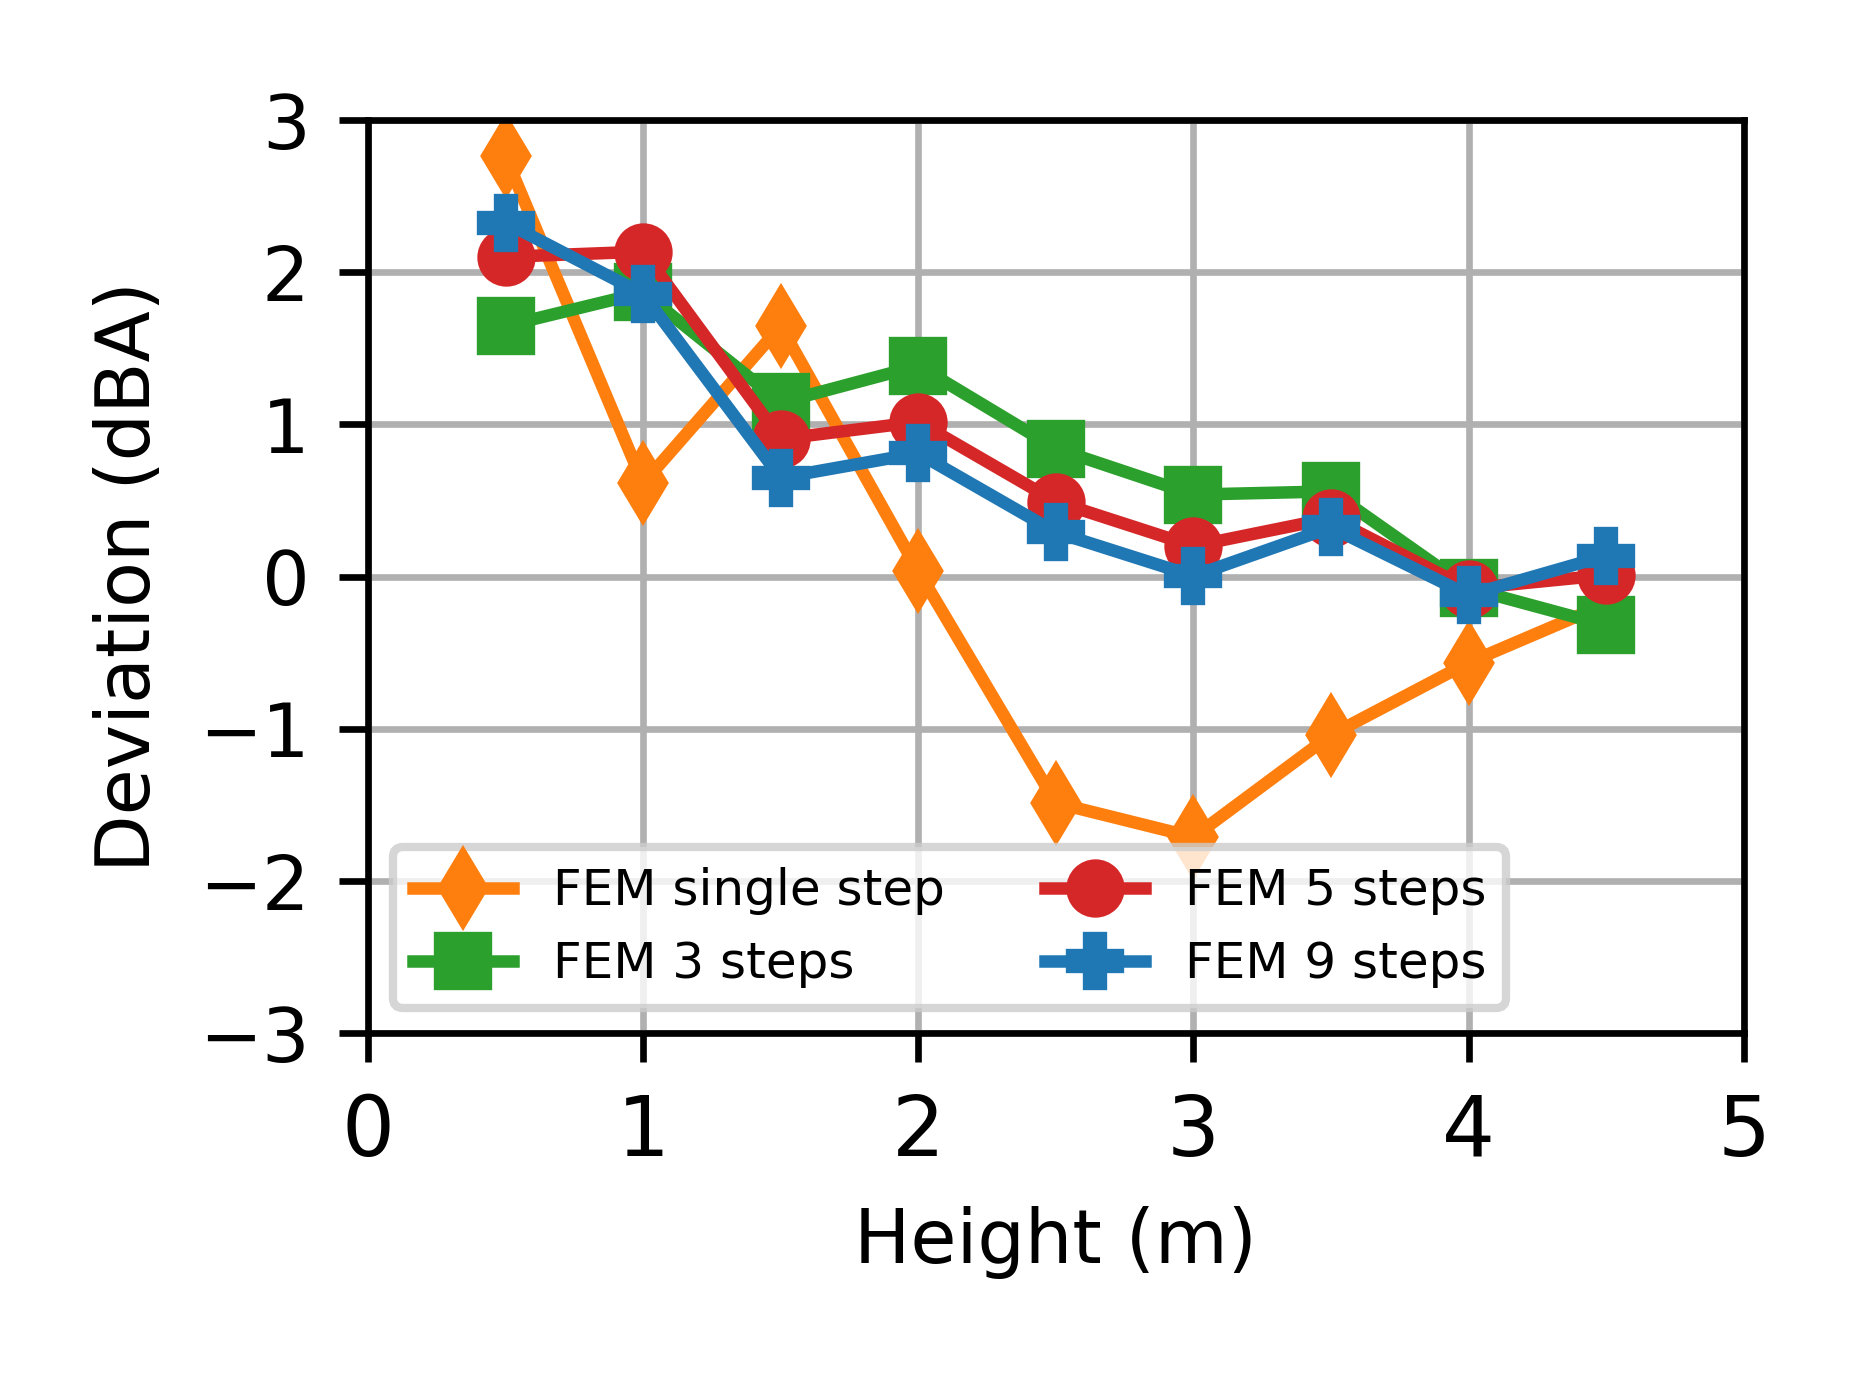
\includegraphics[width=0.49\textwidth]{fig/chap5/freq_steps/overall_SPL/pos_f_deviation.png}
		\caption{\SI{10}{\centi\meter} from the carbody}
	\end{subfigure}
	\caption{Comparison between simulation (full lines) using different intermediate frequency steps per one-third octave band and measurement (dashed lines) over the height at various measurement positions. Left: Overall SPL in dBA ref \SI{20}{\micro\pascal}; Right: Deviation between simulation and measurement results.}
	\label{fig:overall_SPL_freq_steps}
\end{figure}

\Cref{fig:overall_SPL_freq_steps} shows the overall A-weighted sound pressure level distribution obtained by using different intermediate frequency steps compared to the measurement.
As can be seen from the figures, at most of the microphone locations the simulation using nine frequency steps per one-third octave band shows the closest fit to the measurement while the results obtained by using three or five intermediate steps are also in the same range, but with a slightly greater deviation.
When using only one single frequency step, a noticeable difference to the measured SPL curve at \SIrange{2}{4}{\meter} height can be observed. This is also the range of the height in which for several one-third octave band center frequencies the sinks in sound pressure level curves are located, as previously shown in \cref{fig:third_octave_over_height}.

\begin{table}
	\caption{Mean relative error in overall SPL and total computation time using different intermediate frequency steps per one third octave band.}
	\label{tab:freq_steps_MRE}
	\centering
	\begin{tabular}{ccc}
		\toprule
		Number of intermediate steps & MRE in overall SPL (dB) & Total computation time (h) \\ 
		\midrule
		1  & 1.10 & 4.5 \\ 
		3  & 0.82 & 10 \\
		5  & 0.76 & 15 \\
		9  & 0.73 & 27 \\
		\bottomrule
	\end{tabular}
\end{table}

\Cref{tab:freq_steps_MRE} shows the mean relative error in terms of the overall A-weight sound pressure level to the measurement obtained by using different intermediate frequency steps per one-third octave band. Further, the total computation time for all 14 one-third octave bands covering \SIrange{100}{2000}{\hertz} is also shown in the same table. As expected, the more intermediate steps per one-third octave band are used, the better the approximation to the measured results. On the other hand, it can be seen that the convergence rate of the mean relative error is getting slower with increasing intermediate steps, which means upon a certain degree of frequency resolution, a better approximation cannot be achieved by simply using more intermediate frequency steps per one-third octave band. Another important aspect of choosing the proper number of intermediate frequency steps is the total computation time of the simulation, which increases linearly with the number of frequency steps. For our finite element model, choosing five intermediate steps per one-third octave band would be a good compromise between accuracy and computational effort, since it has a similar mean relative error in terms of overall sound pressure level as the initial setup with nine intermediate steps but saves up almost 50 percent of the computation time.

From the results shown in this section, it can be concluded that the number of intermediate frequency steps used per one-third octave band affects the prediction accuracy of the finite element model. In the low frequency range, using one single frequency step to resolve the one-third octave band is sufficient while with increasing frequency, more intermediate steps are needed to obtain a good approximation to the measurement result. For the investigated finite element model, there is no noticeable difference in terms of overall sound pressure level between the simulation results obtained by using three, five, and nine intermediate steps, respectively. All three setups show good agreement with the measurement data and differ in their total computation time. For the investigated frequency range from \SIrange{100}{2000}{\hertz}, using five intermediate steps to resolve the one-third octave band is a good compromise between simulation accuracy and computational effort.